\documentclass[10pt,a4paper]{article}
\usepackage[utf8]{inputenc}
\usepackage{amsmath}
\usepackage{amsfonts}
\usepackage{graphicx}
\usepackage{amssymb}
\usepackage[left=2cm,right=2cm,top=2cm,bottom=2cm]{geometry}
\usepackage{tikz}
\usepackage{pgfplots}
\usetikzlibrary{shapes,arrows,positioning}
\title{Théorie des communications numériques}
\date{}
\renewcommand{\contentsname}{Sommaire}
\usepackage{setspace}
\onehalfspacing
\setlength{\parindent}{0pt}

\pgfmathdeclarefunction{qfunc}{1}{%
  \pgfmathparse{1/(1 + exp(0.717*#1 + 0.416*#1*#1))}%
}

\begin{document}

\section*{Introduction}

\subsection*{Purpose of a Communication System}
Un système de communication a pour objectif de transmettre des signaux porteurs d'information d'un point à un autre dans l'espace. Les informations peuvent être de différentes natures : signaux électriques, sonores, lumineux, etc.

\subsection*{Communication Chain}
La chaîne de communication est composée de trois éléments principaux :
\begin{itemize}
    \item \textbf{Émetteur} : Transforme le signal numérique en un signal physique (par exemple, un signal électrique ou une onde électromagnétique) qui peut être transmis sur le canal.
    \item \textbf{Canal} : Milieu physique de transmission. Il peut avoir différentes propriétés physiques et peut causer des erreurs (bruit, perte d'information, etc.).
    \item \textbf{Récepteur} : Transforme le signal reçu en une reconstruction du signal numérique.
\end{itemize}

\subsection*{Exemple de Chaîne de Communication}

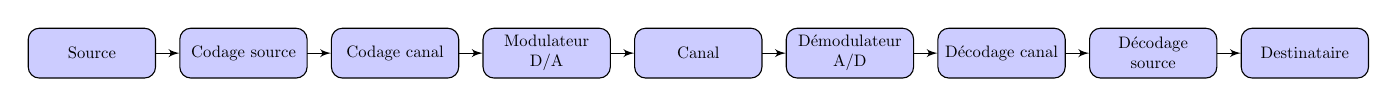
\begin{tikzpicture}[node distance=0.5cm, auto, scale=0.6, transform shape]
    \tikzstyle{block} = [rectangle, draw, fill=blue!20, text width=7em, text centered, rounded corners, minimum height=3em]
    \tikzstyle{line} = [draw, -latex']

    \node[block] (source) {Source};
    \node[block, right=of source] (sourcecoding) {Codage source};
    \node[block, right=of sourcecoding] (channelcoding) {Codage canal};
    \node[block, right=of channelcoding] (modulator) {Modulateur D/A};
    \node[block, right=of modulator] (channel) {Canal};
    \node[block, right=of channel] (demodulator) {Démodulateur A/D};
    \node[block, right=of demodulator] (channeldecoding) {Décodage canal};
    \node[block, right=of channeldecoding] (sourcedecoding) {Décodage source};
    \node[block, right=of sourcedecoding] (recipient) {Destinataire};

    \path[line] (source) -- (sourcecoding);
    \path[line] (sourcecoding) -- (channelcoding);
    \path[line] (channelcoding) -- (modulator);
    \path[line] (modulator) -- (channel);
    \path[line] (channel) -- (demodulator);
    \path[line] (demodulator) -- (channeldecoding);
    \path[line] (channeldecoding) -- (sourcedecoding);
    \path[line] (sourcedecoding) -- (recipient);
\end{tikzpicture}


\subsection*{Théorie de l'Information}
La théorie de l'information traite de la quantification, du stockage et de la communication de l'information. Elle est essentielle pour comprendre comment les données sont compressées et protégées contre les erreurs de transmission.

\subsubsection*{Codage de Source}
Le codage de source vise à réduire le nombre de symboles dans un message au minimum nécessaire pour représenter l'information. Cela permet de compresser les données et d'optimiser l'utilisation de la bande passante.

\subsubsection*{Codage de Canal}
Le codage de canal introduit sélectivement des bits redondants pour détecter et corriger les erreurs de transmission. Cela améliore la fiabilité de la communication.

\section*{Signal Theory}

\subsection*{Signaux Discrets et Continus}
Un signal est dit \textbf{discret} si son support temporel est fini ou dénombrable. Par exemple, un signal numérique est un signal discret.

Un signal est dit \textbf{continu} si son support temporel est constitué d'intervalles de $\mathbb{R}$. Par exemple, un signal analogique est un signal continu.

\subsubsection*{Exemple de Signal Discret}
Un signal discret peut être défini par des échantillons $x_k = x(k)$ et une période $T$ :
\[ x(t) = \sum_{k \in \mathbb{Z}} x_k \delta(t - kT) \]

\subsection*{Signaux Déterministes et Stochastiques}
Un signal est dit \textbf{déterministe} si sa forme d'onde est connue. Par exemple, une sinusoïde d'amplitude, de phase et de fréquence fixes.

Un signal est dit \textbf{stochastique} s'il est perturbé par du bruit et devient imprévisible. Par exemple, un signal perturbé par du bruit blanc gaussien.

\subsection*{Transformée de Fourier}
La transformée de Fourier est un outil mathématique qui permet de décomposer un signal en ses composantes fréquentielles. Pour un signal continu $x(t)$, la transformée de Fourier est donnée par :
\[ X(f) = \int_{-\infty}^{+\infty} x(t) e^{-2j\pi ft} \, dt \]

\subsection*{Exemple de Transformée de Fourier}
Pour un signal rectangulaire $x(t) = \text{rect}(t)$, la transformée de Fourier est :
\[ X(f) = \text{sinc}(f) \]

\subsection*{Signaux Stochastiques}
Les signaux stochastiques sont des signaux aléatoires. Leur analyse nécessite des outils statistiques comme la densité spectrale de puissance (PSD) et l'autocorrélation.

\subsubsection*{Exemple de Signal Stochastique}
Un processus gaussien est un exemple de signal stochastique. Chaque échantillon $X(t, \omega)$ est une variable aléatoire distribuée selon une loi normale :
\[ f_X(t) = \frac{1}{\sigma \sqrt{2\pi}} e^{-\frac{1}{2}\left(\frac{t-\mu}{\sigma}\right)^2} \]

\subsection*{Bruit Blanc Gaussien Additif (AWGN)}
Le bruit blanc gaussien additif est un modèle de bruit couramment utilisé dans les systèmes de communication. Il est caractérisé par une densité spectrale de puissance constante et une distribution gaussienne.

\subsubsection*{Propriétés du AWGN}
- Moyenne nulle : $\mathbb{E}[n(t)] = 0$
- Variance : $\sigma_B^2 = \frac{N_0}{2}$
- Densité spectrale de puissance : $\frac{N_0}{2}$

\subsection*{Capacité du Canal}
La capacité d'un canal est la limite théorique supérieure du débit auquel l'information peut être transmise de manière fiable sur un canal de communication. Pour un canal AWGN, la capacité est donnée par le théorème de Shannon-Hartley :
\[ C = B_T \log_2(1 + \text{SNR}) \]
où $B_T$ est la bande passante totale et SNR est le rapport signal sur bruit.

\subsection*{Ajout : Interférence Entre Symboles (ISI)}
L'interférence entre symboles (ISI) se produit lorsque des symboles consécutifs interfèrent les uns avec les autres. Cela peut être causé par une limitation de la bande passante ou par des distorsions introduites par le canal.

\subsubsection*{Effet de l'ISI}
L'ISI peut entraîner des erreurs de détection au niveau du récepteur. Pour minimiser l'ISI, des techniques comme le critère de Nyquist et le filtrage en cosinus surélevé sont utilisées.

\subsection*{Ajout : Diagramme de l'Oeil}
Le diagramme de l'œil est un outil utilisé pour visualiser l'ISI. Il permet de voir comment les symboles se chevauchent et d'évaluer la qualité de la transmission.

% Ajout d'une illustration pour le diagramme de l'œil
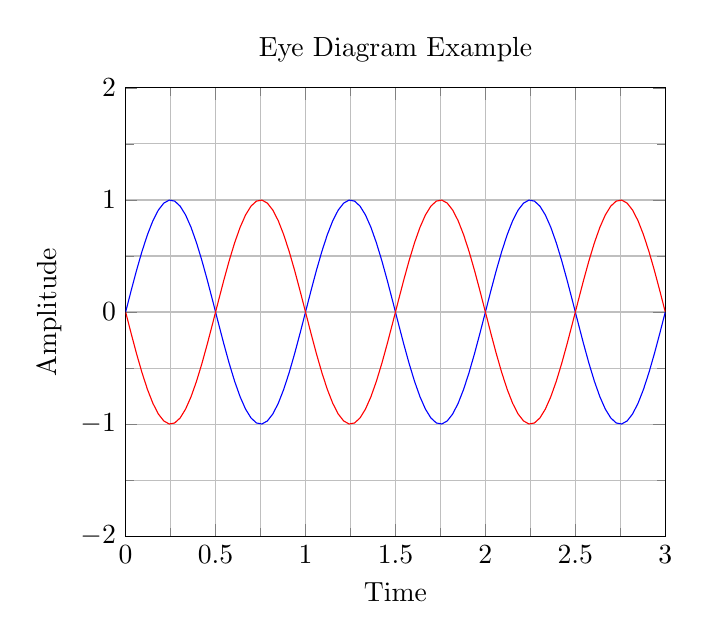
\begin{tikzpicture}
    \begin{axis}[
        xlabel=Time,
        ylabel=Amplitude,
        title=Eye Diagram Example,
        xmin=0, xmax=3,
        ymin=-2, ymax=2,
        grid=both,
        minor tick num=1,
    ]
    \addplot[blue, domain=0:3, samples=100] {sin(2*pi*deg(x))};
    \addplot[red, domain=0:3, samples=100] {sin(2*pi*deg(x) + 180)};
    \end{axis}
\end{tikzpicture}

\section*{Emitter : Transmission en Bande de Base}

\subsection*{Introduction à la Transmission en Bande de Base}
La transmission en bande de base consiste à transmettre un signal numérique sans modulation sur une porteuse. Cela signifie que le signal occupe une bande de fréquences autour de zéro.

\subsubsection*{Objectifs}
\begin{itemize}
    \item Transmettre des données numériques de manière efficace.
    \item Adapter le signal au canal de transmission.
\end{itemize}

\subsection*{Codage Binaire}
Le codage binaire est une méthode de représentation des bits sous forme de signaux électriques.

\subsubsection*{Non-Return to Zero (NRZ)}
Dans le codage NRZ, les bits sont représentés par des niveaux de tension constants pendant toute la durée du bit.
\begin{itemize}
    \item 0 : tension basse (par exemple, 0V)
    \item 1 : tension haute (par exemple, +V)
\end{itemize}

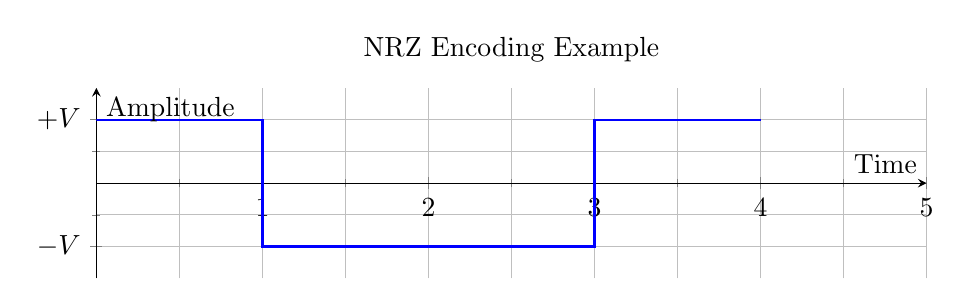
\begin{tikzpicture}
    \begin{axis}[
        width=\textwidth,
        height=4cm,
        xlabel=Time,
        ylabel=Amplitude,
        title=NRZ Encoding Example,
        xmin=0, xmax=5,
        ymin=-1.5, ymax=1.5,
        grid=both,
        minor tick num=1,
        xtick={0,1,2,3,4,5},
        ytick={-1,0,1},
        yticklabels={$-V$, $0$, $+V$},
        axis lines=middle,
    ]
    \addplot[blue, thick, const plot mark right, samples at={0,1,2,3,4}] coordinates {
        (0, 1)
        (1, 1)
        (2, -1)
        (3, -1)
        (4, 1)
    };
    \end{axis}
\end{tikzpicture}

\subsubsection*{Return to Zero (RZ)}
Dans le codage RZ, le signal retourne à zéro après chaque bit.
\begin{itemize}
    \item 0 : tension passe brièvement à basse puis revient à zéro.
    \item 1 : tension passe brièvement à haute puis revient à zéro.
\end{itemize}

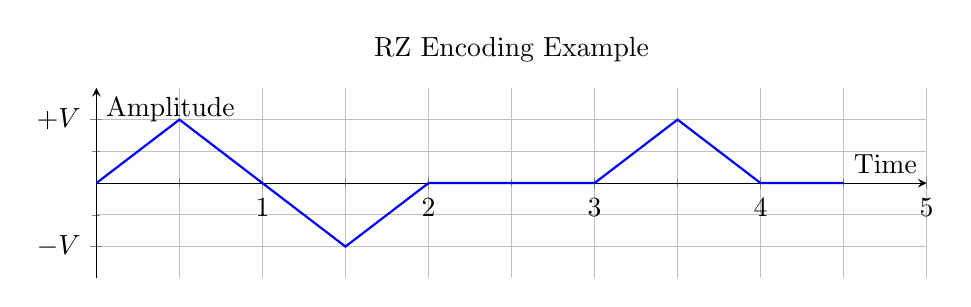
\begin{tikzpicture}
    \begin{axis}[
        width=\textwidth,
        height=4cm,
        xlabel=Time,
        ylabel=Amplitude,
        title=RZ Encoding Example,
        xmin=0, xmax=5,
        ymin=-1.5, ymax=1.5,
        grid=both,
        minor tick num=1,
        xtick={0,1,2,3,4,5},
        ytick={-1,0,1},
        yticklabels={$-V$, $0$, $+V$},
        axis lines=middle,
    ]
    \addplot[blue, thick, samples at={0,0.5,1,1.5,2,2.5,3,3.5,4,4.5}] coordinates {
        (0, 0)
        (0.5, 1)
        (1, 0)
        (1.5, -1)
        (2, 0)
        (2.5, 0)
        (3, 0)
        (3.5, 1)
        (4, 0)
        (4.5, 0)
    };
    \end{axis}
\end{tikzpicture}

\subsection*{Codage M-aire}
Le codage M-aire utilise un alphabet de taille M pour représenter les données. Chaque symbole représente $\log_2(M)$ bits.

\subsubsection*{Exemple de Codage 4-aire}
Un exemple de codage 4-aire utilise les niveaux de tension suivants pour représenter les paires de bits :
\begin{itemize}
    \item 00 : -3V
    \item 01 : -1V
    \item 10 : +1V
    \item 11 : +3V
\end{itemize}

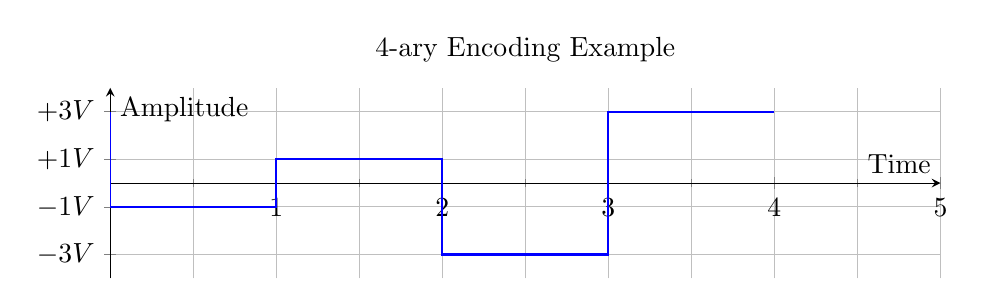
\begin{tikzpicture}
    \begin{axis}[
        width=\textwidth,
        height=4cm,
        xlabel=Time,
        ylabel=Amplitude,
        title=4-ary Encoding Example,
        xmin=0, xmax=5,
        ymin=-4, ymax=4,
        grid=both,
        minor tick num=1,
        xtick={0,1,2,3,4,5},
        ytick={-3,-1,0,1,3},
        yticklabels={$-3V$, $-1V$, $0$, $+1V$, $+3V$},
        axis lines=middle,
    ]
    \addplot[blue, thick, const plot mark right, samples at={0,1,2,3,4}] coordinates {
        (0, 3)
        (1, -1)
        (2, 1)
        (3, -3)
        (4, 3)
    };
    \end{axis}
\end{tikzpicture}

\subsection*{Code de Gray}
Le code de Gray est un système de codage binaire où deux valeurs successives ne diffèrent que par un seul bit. Cela réduit la probabilité d'erreur lors de la transmission.

\subsubsection*{Exemple de Code de Gray}
Voici un exemple de code de Gray pour 3 bits :

\begin{tabular}{|c|c|c|}
    \hline
    Valeur Décimale & Code Binaire & Code de Gray \\
    \hline
    0 & 000 & 000 \\
    1 & 001 & 001 \\
    2 & 010 & 011 \\
    3 & 011 & 010 \\
    4 & 100 & 110 \\
    5 & 101 & 111 \\
    6 & 110 & 101 \\
    7 & 111 & 100 \\
    \hline
\end{tabular}

\subsection*{Filtrage d'Émission}
Le filtrage d'émission modifie la forme du signal pour l'adapter au canal de transmission. Cela permet de limiter la bande passante et de réduire l'interférence entre symboles (ISI).

\subsubsection*{Exemple de Filtrage}
Un filtre en cosinus surélevé est souvent utilisé pour limiter l'ISI. La réponse impulsionnelle d'un filtre en cosinus surélevé est donnée par :
\[ h(t) = \frac{\sin(\pi t / T)}{(\pi t / T)} \cdot \frac{\cos(\alpha \pi t / T)}{1 - (2 \alpha t / T)^2} \]
où $\alpha$ est le facteur de roll-off.

\subsection*{Spectre d'Occupation}
Le spectre d'occupation décrit comment le signal occupe la bande de fréquences. Il est important de limiter cette occupation pour éviter les interférences avec d'autres signaux.

\subsubsection*{Exemple de Spectre}
Pour un signal NRZ, le spectre est donné par :
\[ S(f) = A^2 T_s \text{sinc}^2(f T_s) \]

\subsection*{Interférence Entre Symboles (ISI)}
L'ISI se produit lorsque les symboles consécutifs interfèrent les uns avec les autres. Cela peut être causé par une limitation de la bande passante ou des distorsions introduites par le canal.

\subsubsection*{Critère de Nyquist}
Le critère de Nyquist stipule que pour éviter l'ISI, la réponse globale du système doit être nulle à tous les instants de décision sauf à l'instant central.

\subsection*{Diagramme de l'Œil}
Le diagramme de l'œil est un outil utilisé pour visualiser l'ISI. Il permet de voir comment les symboles se chevauchent et d'évaluer la qualité de la transmission.

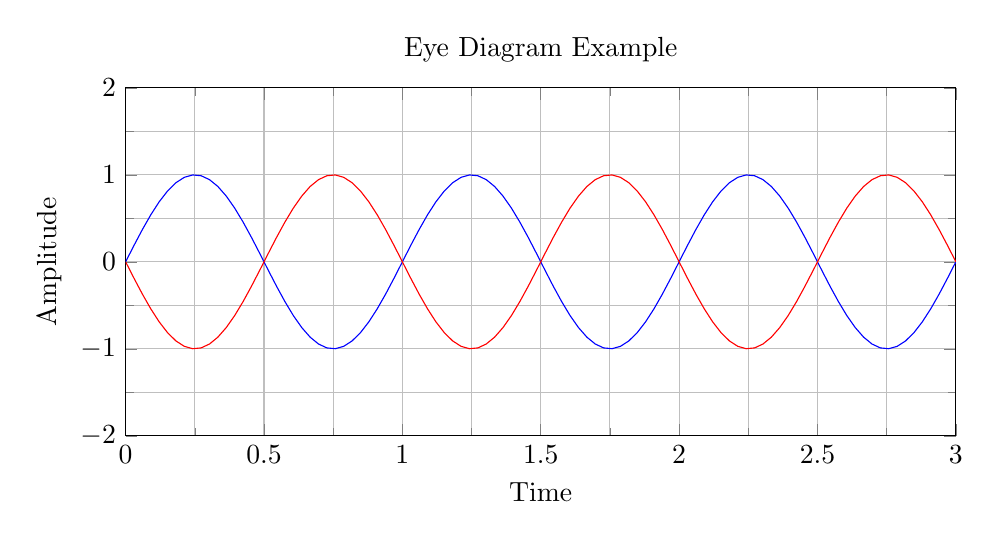
\begin{tikzpicture}
    \begin{axis}[
        width=\textwidth,
        height=6cm,
        xlabel=Time,
        ylabel=Amplitude,
        title=Eye Diagram Example,
        xmin=0, xmax=3,
        ymin=-2, ymax=2,
        grid=both,
        minor tick num=1,
    ]
    \addplot[blue, domain=0:3, samples=100] {sin(2*pi*deg(x))};
    \addplot[red, domain=0:3, samples=100] {sin(2*pi*deg(x) + 180)};
    \end{axis}
\end{tikzpicture}

\subsection*{Échantillonnage}
L'échantillonnage transforme un signal continu en un signal discret. Cela permet de traiter le signal numériquement.

\subsubsection*{Théorème d'Échantillonnage de Nyquist-Shannon}
Pour reconstruire parfaitement un signal continu à partir de ses échantillons, la fréquence d'échantillonnage doit être au moins deux fois la fréquence maximale du signal.

\subsection*{Décision}
La décision consiste à déterminer quel symbole a été transmis en fonction de l'échantillon reçu. Cela implique souvent un seuil de décision pour distinguer entre les différents niveaux de tension.

\subsection*{Probabilité d'Erreur}
La probabilité d'erreur dépend du rapport signal sur bruit (SNR) et du type de codage utilisé.

\subsubsection*{Exemple de Probabilité d'Erreur pour NRZ}
Pour un signal NRZ en présence de bruit blanc gaussien additif (AWGN), la probabilité d'erreur est donnée par :
\[ P_e = Q\left(\sqrt{\frac{2E_b}{N_0}}\right) \]
où \(E_b\) est l'énergie par bit et \(N_0\) est la densité spectrale de puissance du bruit.

\subsection*{Filtrage Adapté}
Le filtre adapté est utilisé pour maximiser le rapport signal sur bruit à l'instant de décision.

\subsubsection*{Réponse Impulsionnelle du Filtre Adapté}
La réponse impulsionnelle du filtre adapté est donnée par :
\[ h(t) = s(T - t) \]
où \(s(t)\) est le signal reçu.

\subsection*{Représentation Vectorielle}
La représentation vectorielle des signaux permet de simplifier l'analyse des systèmes de communication. Chaque symbole peut être représenté comme un vecteur dans un espace de signal.

\subsection*{Modulation Numérique}
La modulation numérique adapte le signal au canal physique en utilisant une porteuse.

\subsubsection*{Exemple de Modulation QPSK}
La modulation QPSK (Quadrature Phase Shift Keying) utilise quatre points de constellation pour représenter deux bits par symbole.

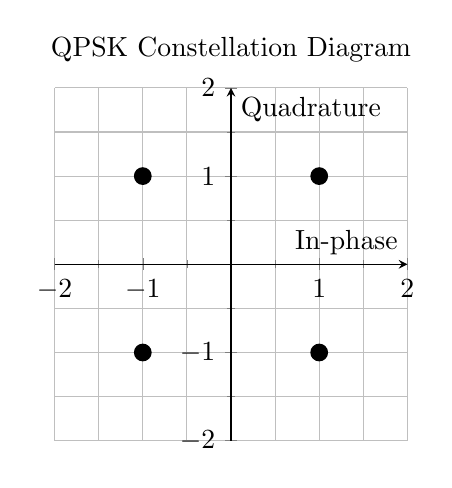
\begin{tikzpicture}
    \begin{axis}[
        width=0.5\textwidth,
        height=0.5\textwidth,
        xlabel=In-phase,
        ylabel=Quadrature,
        title=QPSK Constellation Diagram,
        xmin=-2, xmax=2,
        ymin=-2, ymax=2,
        grid=both,
        minor tick num=1,
        axis lines=middle,
    ]
    \addplot[only marks, mark=*, mark size=3pt] coordinates {
        (1, 1)
        (-1, 1)
        (-1, -1)
        (1, -1)
    };
    \end{axis}
\end{tikzpicture}

\subsection*{Filtrage des Signaux Modulés}
Le filtrage des signaux modulés permet de limiter la bande passante et de réduire les interférences.

\subsection*{Taux d'Erreur Binaire (BER) et Taux d'Erreur Symbole (SER)}
Le BER et le SER sont des métriques importantes pour évaluer la performance d'un système de communication.

\subsubsection*{Exemple de Calcul de BER}
Pour un signal QPSK en présence de bruit AWGN, le BER est donné par :
\[ P_b = Q\left(\sqrt{\frac{2E_b}{N_0}}\right) \]

\section*{Channel}

\subsection*{Caractéristiques du Canal}
Le canal est le milieu physique par lequel le signal se propage de l'émetteur au récepteur. Il peut introduire des distorsions et du bruit, ce qui affecte la qualité du signal reçu.

\subsubsection*{Types de Canaux}
\begin{itemize}
    \item \textbf{Canal filaire} : Câbles coaxiaux, paires torsadées, fibres optiques.
    \item \textbf{Canal sans fil} : Ondes radio, micro-ondes, infrarouges.
\end{itemize}

\subsubsection*{Bruit et Distorsions}
Le canal peut introduire :
\begin{itemize}
    \item \textbf{Bruit} : Perturbations aléatoires qui altèrent le signal. Le bruit blanc gaussien additif (AWGN) est un modèle commun.
    \item \textbf{Distorsion} : Déformation du signal due à des limitations de bande passante ou à des non-linéarités.
\end{itemize}

\subsection*{Modélisation du Canal}
Un canal peut être modélisé par sa réponse impulsionnelle \( h_c(t) \). Pour un canal linéaire, la sortie \( y(t) \) est donnée par la convolution du signal d'entrée \( x(t) \) avec \( h_c(t) \) :
\[ y(t) = x(t) * h_c(t) + n(t) \]
où \( n(t) \) représente le bruit.

\subsubsection*{Exemple de Réponse Impulsionnelle}
Pour un canal idéal sans distorsion, \( h_c(t) = \delta(t) \), où \( \delta(t) \) est l'impulsion de Dirac.

\subsection*{Capacité du Canal}
La capacité du canal est la quantité maximale d'information qui peut être transmise de manière fiable à travers le canal. Pour un canal AWGN, la capacité est donnée par le théorème de Shannon-Hartley :
\[ C = B \log_2(1 + \text{SNR}) \]
où \( B \) est la bande passante et SNR est le rapport signal sur bruit.

\subsection*{Exemple de Canal Réel}
Pour un canal de téléphone, la bande passante est généralement limitée à 300 Hz - 3400 Hz, ce qui limite la capacité de transmission des données.

\section*{Receiver : Intersymbol Interference (ISI)}

\subsection*{Introduction à l'ISI}
L'interférence entre symboles (ISI) se produit lorsque les symboles consécutifs dans un signal se chevauchent, ce qui peut entraîner des erreurs de détection au niveau du récepteur.

\subsubsection*{Causes de l'ISI}
\begin{itemize}
    \item Limitation de la bande passante du canal.
    \item Distorsion introduite par le canal.
    \item Mauvaise synchronisation entre l'émetteur et le récepteur.
\end{itemize}

\subsection*{Effets de l'ISI}
L'ISI peut entraîner des erreurs dans la détection des symboles, réduisant ainsi la fiabilité de la communication.

\subsection*{Critère de Nyquist pour l'ISI}
Pour éviter l'ISI, le critère de Nyquist stipule que la réponse globale du système doit être nulle à tous les instants de décision, sauf à l'instant central. Mathématiquement, cela signifie que :
\[ g(nT_s) =
  \begin{cases}
   1 & \text{si } n = 0 \\
   0 & \text{si } n \neq 0
  \end{cases}
\]
où \( g(t) \) est la réponse globale du système et \( T_s \) est la période des symboles.

\subsection*{Diagramme de l'Œil}
Le diagramme de l'œil est un outil graphique utilisé pour évaluer la qualité d'un signal en présence d'ISI. Il est généré en superposant des segments du signal sur une période de symbole.

\subsubsection*{Interprétation du Diagramme de l'Œil}
\begin{itemize}
    \item \textbf{Ouverture de l'œil} : Une grande ouverture indique une faible ISI.
    \item \textbf{Fermeture de l'œil} : Une fermeture de l'œil indique une ISI significative.
\end{itemize}

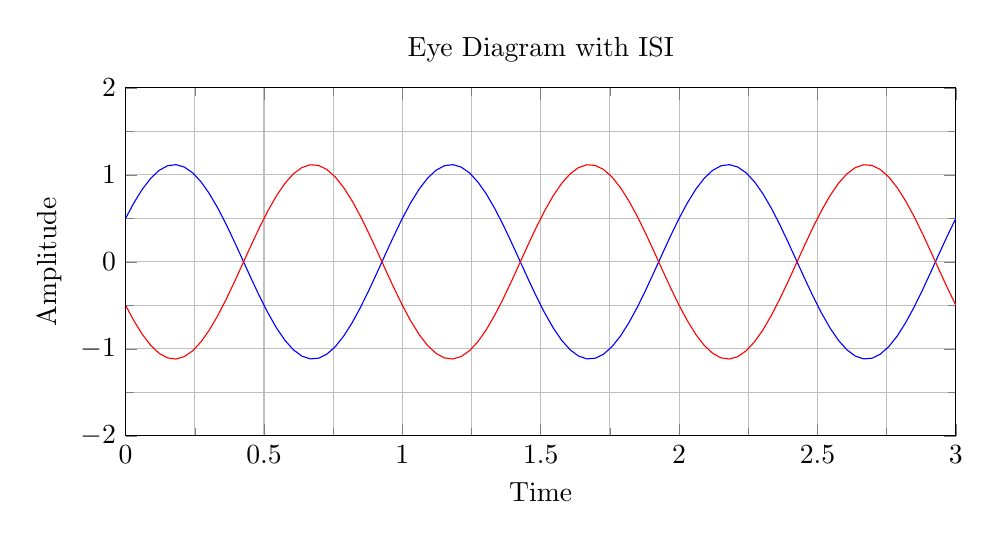
\begin{tikzpicture}
    \begin{axis}[
        width=\textwidth,
        height=6cm,
        xlabel=Time,
        ylabel=Amplitude,
        title=Eye Diagram with ISI,
        xmin=0, xmax=3,
        ymin=-2, ymax=2,
        grid=both,
        minor tick num=1,
    ]
    \addplot[blue, domain=0:3, samples=100] {sin(2*pi*deg(x)) + 0.5*sin(2*pi*deg(x) + 90)};
    \addplot[red, domain=0:3, samples=100] {sin(2*pi*deg(x) + 180) + 0.5*sin(2*pi*deg(x) + 270)};
    \end{axis}
\end{tikzpicture}

\subsection*{Filtrage en Cosinus Surélevé}
Le filtrage en cosinus surélevé est une technique utilisée pour réduire l'ISI. La réponse en fréquence d'un filtre en cosinus surélevé est donnée par :
\[ H(f) =
  \begin{cases}
   1 & \text{si } |f| < \frac{1 - \alpha}{2T_s} \\
   \frac{1}{2} \left[1 + \cos\left(\frac{\pi T_s}{\alpha} \left(|f| - \frac{1 - \alpha}{2T_s}\right)\right)\right] & \text{si } \frac{1 - \alpha}{2T_s} < |f| < \frac{1 + \alpha}{2T_s} \\
   0 & \text{sinon}
  \end{cases}
\]
où \( \alpha \) est le facteur de roll-off.

\subsubsection*{Effet du Filtrage en Cosinus Surélevé}
Un filtre en cosinus surélevé permet de limiter la bande passante du signal tout en réduisant l'ISI.

\subsection*{Échantillonnage}
L'échantillonnage est le processus de conversion d'un signal continu en un signal discret. Cela permet de traiter le signal numériquement.

\subsubsection*{Théorème d'Échantillonnage de Nyquist-Shannon}
Pour reconstruire parfaitement un signal continu à partir de ses échantillons, la fréquence d'échantillonnage doit être au moins deux fois la fréquence maximale du signal.

\subsection*{Décision}
La décision consiste à déterminer quel symbole a été transmis en fonction de l'échantillon reçu. Cela implique souvent un seuil de décision pour distinguer entre les différents niveaux de tension.

\subsubsection*{Seuil de Décision}
Pour un signal binaire, le seuil de décision est généralement fixé à mi-chemin entre les niveaux de tension représentant les bits 0 et 1.

\subsection*{Probabilité d'Erreur}
La probabilité d'erreur dépend du rapport signal sur bruit (SNR) et du type de codage utilisé.

\subsubsection*{Exemple de Probabilité d'Erreur pour NRZ}
Pour un signal NRZ en présence de bruit blanc gaussien additif (AWGN), la probabilité d'erreur est donnée par :
\[ P_e = Q\left(\sqrt{\frac{2E_b}{N_0}}\right) \]
où \( E_b \) est l'énergie par bit et \( N_0 \) est la densité spectrale de puissance du bruit.

\subsection*{Filtre Adapté}
Le filtre adapté est utilisé pour maximiser le rapport signal sur bruit à l'instant de décision.

\subsubsection*{Réponse Impulsionnelle du Filtre Adapté}
La réponse impulsionnelle du filtre adapté est donnée par :
\[ h(t) = s(T - t) \]
où \( s(t) \) est le signal reçu.

\subsection*{Représentation Vectorielle}
La représentation vectorielle des signaux permet de simplifier l'analyse des systèmes de communication. Chaque symbole peut être représenté comme un vecteur dans un espace de signal.

\subsection*{Modulation Numérique}
La modulation numérique adapte le signal au canal physique en utilisant une porteuse.

\subsubsection*{Exemple de Modulation QPSK}
La modulation QPSK (Quadrature Phase Shift Keying) utilise quatre points de constellation pour représenter deux bits par symbole.

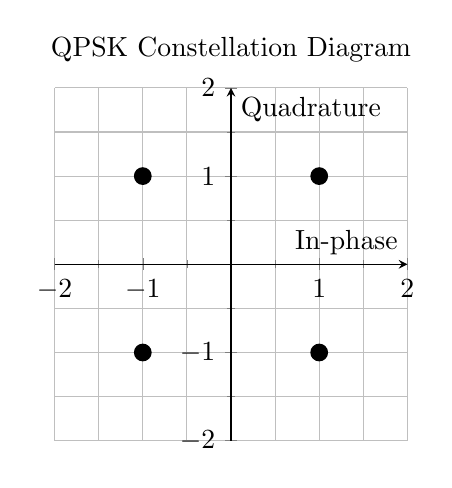
\begin{tikzpicture}
    \begin{axis}[
        width=0.5\textwidth,
        height=0.5\textwidth,
        xlabel=In-phase,
        ylabel=Quadrature,
        title=QPSK Constellation Diagram,
        xmin=-2, xmax=2,
        ymin=-2, ymax=2,
        grid=both,
        minor tick num=1,
        axis lines=middle,
    ]
    \addplot[only marks, mark=*, mark size=3pt] coordinates {
        (1, 1)
        (-1, 1)
        (-1, -1)
        (1, -1)
    };
    \end{axis}
\end{tikzpicture}

\subsection*{Filtrage des Signaux Modulés}
Le filtrage des signaux modulés permet de limiter la bande passante et de réduire les interférences.

\subsection*{Taux d'Erreur Binaire (BER) et Taux d'Erreur Symbole (SER)}
Le BER et le SER sont des métriques importantes pour évaluer la performance d'un système de communication.

\subsubsection*{Exemple de Calcul de BER}
Pour un signal QPSK en présence de bruit AWGN, le BER est donné par :
\[ P_b = Q\left(\sqrt{\frac{2E_b}{N_0}}\right) \]

\section*{Raised-Cosine Filter}

\subsection*{Introduction}
Le filtre en cosinus surélevé est largement utilisé dans les systèmes de communication pour réduire l'interférence entre symboles (ISI). Il permet de limiter la bande passante du signal tout en préservant une bonne séparation entre les symboles.

\subsection*{Réponse en Fréquence}
La réponse en fréquence \( H(f) \) d'un filtre en cosinus surélevé est donnée par :

\[
H(f) =
  \begin{cases}
   1 & \text{si } |f| < \frac{1 - \alpha}{2T_s} \\
   \frac{1}{2} \left[1 + \cos\left(\frac{\pi T_s}{\alpha} \left(|f| - \frac{1 - \alpha}{2T_s}\right)\right)\right] & \text{si } \frac{1 - \alpha}{2T_s} < |f| < \frac{1 + \alpha}{2T_s} \\
   0 & \text{sinon}
  \end{cases}
\]

où :
- \( T_s \) est la période des symboles.
- \( \alpha \) est le facteur de roll-off, avec \( 0 \leq \alpha \leq 1 \).

\subsection*{Réponse Impulsionnelle}
La réponse impulsionnelle \( h(t) \) d'un filtre en cosinus surélevé est donnée par :

\[
h(t) = \frac{\sin\left(\frac{\pi t}{T_s}\right)}{\frac{\pi t}{T_s}} \cdot \frac{\cos\left(\frac{\pi \alpha t}{T_s}\right)}{1 - \left(\frac{2 \alpha t}{T_s}\right)^2}
\]

\subsection*{Effet du Facteur de Roll-Off}
Le facteur de roll-off \( \alpha \) détermine la rapidité de la transition entre la bande passante et la bande atténuée :
- \( \alpha = 0 \) : Le filtre devient un filtre en sinus cardinal (sinc), avec une transition abrupte.
- \( \alpha = 1 \) : Le filtre a une transition plus douce, occupant une bande passante 2 fois plus large.

\subsection*{Illustration de la Réponse en Fréquence}
Voici un exemple de la réponse en fréquence pour différents facteurs de roll-off :

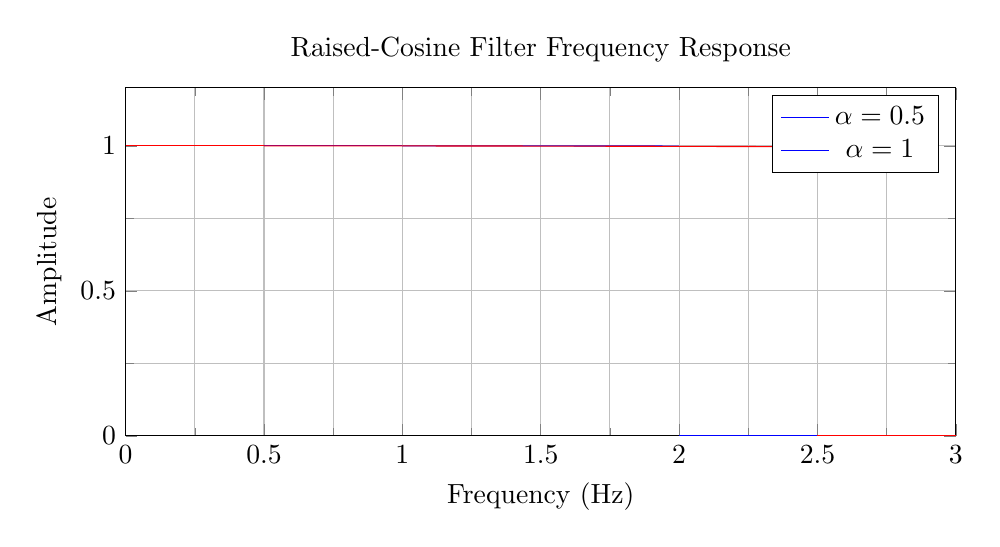
\begin{tikzpicture}
\begin{axis}[
    width=\textwidth,
    height=6cm,
    xlabel=Frequency (Hz),
    ylabel=Amplitude,
    title=Raised-Cosine Filter Frequency Response,
    xmin=0, xmax=3,
    ymin=0, ymax=1.2,
    grid=both,
    minor tick num=1,
]

\addplot[blue, domain=0:1, samples=100] {1};
\addplot[blue, domain=1:2, samples=100] {0.5*(1 + cos(pi*(x-1)))};
\addplot[blue, domain=2:3, samples=100] {0};
\addlegendentry{$\alpha = 0.5$}

\addplot[red, domain=0:0.5, samples=100] {1};
\addplot[red, domain=0.5:2.5, samples=100] {0.5*(1 + cos(pi*(x-0.5)))};
\addplot[red, domain=2.5:3, samples=100] {0};
\addlegendentry{$\alpha = 1$}

\end{axis}
\end{tikzpicture}

\subsection*{Avantages du Filtre en Cosinus Surélevé}
- Réduction de l'ISI.
- Limitation de la bande passante.
- Flexibilité grâce au facteur de roll-off.

\subsection*{Application Pratique}
Le filtre en cosinus surélevé est utilisé dans de nombreux systèmes de communication, tels que :
- Les modems.
- Les systèmes de communication sans fil (Wi-Fi, LTE, etc.).

\subsection*{Exemple Numérique}
Pour un système avec une période de symbole \( T_s = 1 \) microseconde et un facteur de roll-off \( \alpha = 0.5 \), la bande passante nécessaire est de \( 1.5 \) fois la bande passante minimale requise pour transmettre les symboles sans ISI.

\subsection*{Conclusion}
Le filtre en cosinus surélevé est un outil essentiel pour optimiser les performances des systèmes de communication numériques en réduisant l'ISI et en limitant la bande passante utilisée.

\section*{Receiver : Sampling}

\subsection*{Introduction à l'Échantillonnage}
L'échantillonnage est le processus de conversion d'un signal continu en un signal discret. Cela permet de traiter le signal numériquement et de récupérer les informations transmises.

\subsection*{Théorème d'Échantillonnage de Nyquist-Shannon}
Pour reconstruire parfaitement un signal continu à partir de ses échantillons, la fréquence d'échantillonnage \( f_s \) doit être au moins deux fois la fréquence maximale \( f_{\text{max}} \) du signal :
\[ f_s \geq 2f_{\text{max}} \]

\subsection*{Fréquence d'Échantillonnage}
La fréquence d'échantillonnage est généralement choisie pour être supérieure à la fréquence de Nyquist afin de faciliter la reconstruction du signal.

\subsubsection*{Exemple}
Pour un signal dont la fréquence maximale est de 4 kHz, la fréquence d'échantillonnage minimale est de 8 kHz. En pratique, on utilise souvent une fréquence d'échantillonnage de 44.1 kHz pour les CDs audio.

\subsection*{Processus d'Échantillonnage}
L'échantillonnage consiste à prélever des valeurs du signal continu à des intervalles réguliers. Ces valeurs discrètes sont ensuite quantifiées pour être traitées numériquement.

\subsubsection*{Illustration de l'Échantillonnage}
Voici un exemple d'un signal continu et de ses échantillons :

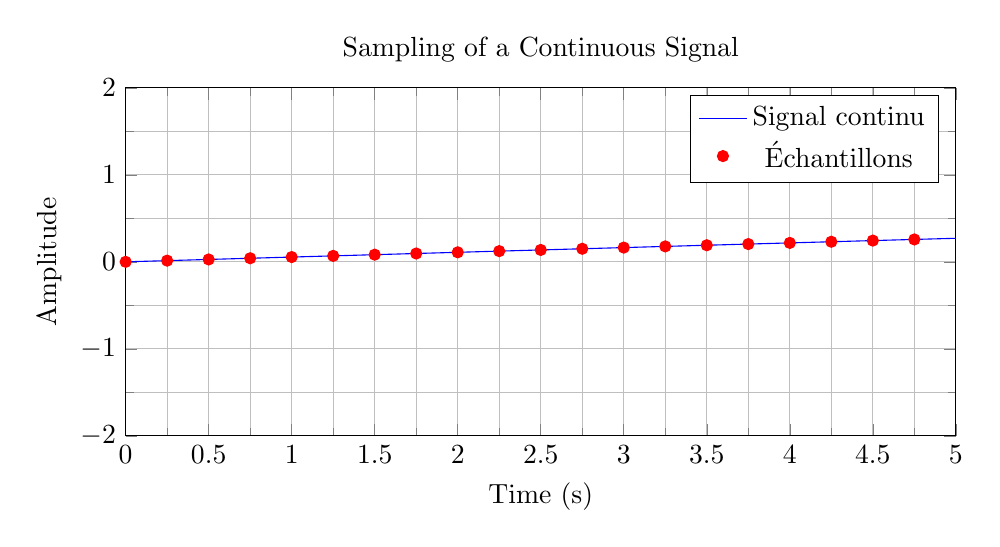
\begin{tikzpicture}
\begin{axis}[
    width=\textwidth,
    height=6cm,
    xlabel=Time (s),
    ylabel=Amplitude,
    title=Sampling of a Continuous Signal,
    xmin=0, xmax=5,
    ymin=-2, ymax=2,
    grid=both,
    minor tick num=1,
]

\addplot[blue, domain=0:5, samples=100] {sin(2*pi*0.5*x)};
\addplot[only marks, mark=*, mark size=2pt, red, samples at={0,0.25,0.5,0.75,1,1.25,1.5,1.75,2,2.25,2.5,2.75,3,3.25,3.5,3.75,4,4.25,4.5,4.75}] {sin(2*pi*0.5*x)};
\legend{Signal continu, Échantillons}

\end{axis}
\end{tikzpicture}

\subsection*{Quantification}
Après l'échantillonnage, les valeurs discrètes sont quantifiées en utilisant un nombre fini de niveaux. Cela introduit une erreur de quantification, qui peut être réduite en augmentant le nombre de bits utilisés pour représenter chaque échantillon.

\subsection*{Erreur de Quantification}
L'erreur de quantification est la différence entre la valeur réelle du signal et la valeur quantifiée. Cette erreur peut être modélisée comme un bruit de quantification.

\subsection*{Reconstruction du Signal}
Pour reconstruire le signal continu à partir des échantillons, on utilise un filtre de reconstruction, tel qu'un filtre passe-bas idéal.

\subsection*{Filtrage Anti-Repliment}
Avant l'échantillonnage, un filtre anti-repliment est utilisé pour éliminer les fréquences supérieures à la moitié de la fréquence d'échantillonnage. Cela évite le phénomène de repliement de spectre (aliasing).

\section*{Receiver : Decision}

\subsection*{Introduction à la Décision}
La décision est le processus par lequel le récepteur détermine quel symbole a été transmis en fonction des échantillons reçus. Cela implique souvent de comparer les échantillons à des seuils de décision.

\subsection*{Seuils de Décision}
Pour un signal binaire, le seuil de décision est généralement fixé à mi-chemin entre les niveaux de tension représentant les bits 0 et 1.

\subsubsection*{Exemple de Seuil de Décision}
Pour un signal NRZ où 0 est représenté par -1V et 1 par +1V, le seuil de décision est fixé à 0V.

\subsection*{Décision en Présence de Bruit}
En présence de bruit, les échantillons peuvent être déviés de leurs valeurs idéales. Le récepteur doit donc prendre une décision en fonction des valeurs reçues et des seuils de décision.

\subsubsection*{Illustration de la Décision en Présence de Bruit}
Voici un exemple de signal binaire bruité et les seuils de décision :

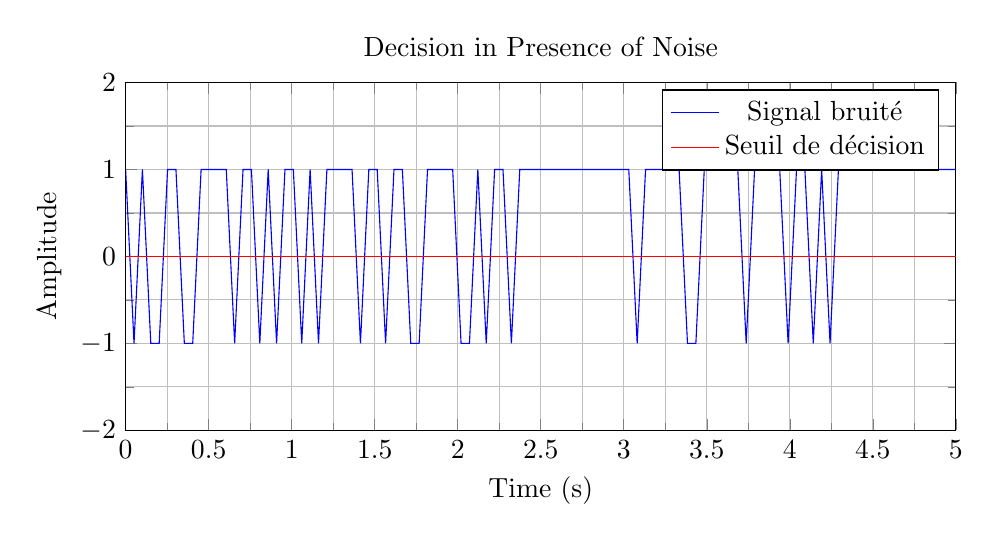
\begin{tikzpicture}
\begin{axis}[
    width=\textwidth,
    height=6cm,
    xlabel=Time (s),
    ylabel=Amplitude,
    title=Decision in Presence of Noise,
    xmin=0, xmax=5,
    ymin=-2, ymax=2,
    grid=both,
    minor tick num=1,
]

\addplot[blue, domain=0:5, samples=100] {sign(sin(2*pi*0.5*x)+0.3*rand)};
\addplot[red, domain=0:5, samples=2] {0};
\legend{Signal bruité, Seuil de décision}

\end{axis}
\end{tikzpicture}

\subsection*{Erreurs de Décision}
Les erreurs de décision se produisent lorsque le bruit ou l'ISI fait que l'échantillon reçu est plus proche du seuil de décision d'un autre symbole.

\subsubsection*{Probabilité d'Erreur}
La probabilité d'erreur dépend du rapport signal sur bruit (SNR) et du type de codage utilisé. Pour un signal binaire en présence de bruit blanc gaussien additif (AWGN), la probabilité d'erreur est donnée par :
\[ P_e = Q\left(\sqrt{\frac{2E_b}{N_0}}\right) \]
où \( E_b \) est l'énergie par bit et \( N_0 \) est la densité spectrale de puissance du bruit.

\subsection*{Décision pour les Signaux M-aires}
Pour les signaux M-aires, le récepteur doit comparer les échantillons reçus à plusieurs seuils de décision pour déterminer quel symbole a été transmis.

\subsubsection*{Exemple de Décision pour un Signal 4-aire}
Pour un signal 4-aire utilisant les niveaux -3V, -1V, +1V et +3V, les seuils de décision sont fixés à -2V, 0V et +2V.

\subsection*{Décision Optimale}
La décision optimale consiste à choisir le symbole qui minimise la probabilité d'erreur. Cela peut être réalisé en utilisant le critère du maximum de vraisemblance (ML).

\subsection*{Maximum de Vraisemblance (ML)}
Le critère de décision ML consiste à choisir le symbole qui maximise la probabilité conditionnelle d'observer l'échantillon reçu, étant donné le symbole transmis.

\subsubsection*{Exemple de Décision ML}
Pour un signal binaire, le récepteur choisit le symbole qui est le plus proche de l'échantillon reçu en termes de distance euclidienne.

\subsection*{Conclusion}
L'échantillonnage et la décision sont des étapes cruciales dans la réception des signaux numériques. Une bonne synchronisation et des seuils de décision appropriés sont essentiels pour minimiser les erreurs et optimiser les performances du système de communication.

\section*{Error Probability}

\subsection*{Introduction}
La probabilité d'erreur est une mesure clé de la performance d'un système de communication. Elle quantifie la probabilité qu'un bit ou un symbole soit incorrectement détecté par le récepteur.

\subsection*{Types d'Erreurs}
Il existe principalement deux types d'erreurs :
\begin{itemize}
    \item **Bit Error** : Erreur sur un bit individuel.
    \item **Symbol Error** : Erreur sur un symbole, qui peut représenter plusieurs bits.
\end{itemize}

\subsection*{Facteurs Influant sur la Probabilité d'Erreur}
Plusieurs facteurs influencent la probabilité d'erreur :
\begin{itemize}
    \item **Rapport Signal sur Bruit (SNR)** : Plus le SNR est élevé, plus la probabilité d'erreur est faible.
    \item **Type de Modulation** : Certaines modulations sont plus robustes aux erreurs que d'autres.
    \item **Interférence Entre Symboles (ISI)** : L'ISI peut augmenter la probabilité d'erreur.
    \item **Bande Passante** : Une bande passante limitée peut introduire des distorsions et augmenter les erreurs.
\end{itemize}

\subsection*{Modèle de Bruit}
Le bruit blanc gaussien additif (AWGN) est un modèle de bruit couramment utilisé pour analyser la probabilité d'erreur. Il est caractérisé par une densité spectrale de puissance constante et une distribution gaussienne.

\subsection*{Fonction Q}
La fonction Q est utilisée pour calculer la probabilité d'erreur en présence de bruit gaussien. Elle est définie comme :
\[ Q(x) = \frac{1}{\sqrt{2\pi}} \int_{x}^{\infty} e^{-t^2/2} \, dt \]

\subsection*{Error Probability of Binary Codes}

\subsubsection*{Binary Phase Shift Keying (BPSK)}
Pour une modulation BPSK, la probabilité d'erreur sur un bit est donnée par :
\[ P_e = Q\left(\sqrt{\frac{2E_b}{N_0}}\right) \]
où \( E_b \) est l'énergie par bit et \( N_0 \) est la densité spectrale de puissance du bruit.

\subsubsection*{Illustration de la Probabilité d'Erreur pour BPSK}
Voici un graphique montrant la probabilité d'erreur pour BPSK en fonction du rapport \( E_b/N_0 \) :

\begin{tikzpicture}
\begin{axis}[
    width=\textwidth,
    height=6cm,
    xlabel=$E_b/N_0$ (dB),
    ylabel=Bit Error Probability ($P_e$),
    title=Bit Error Probability for BPSK,
    xmin=0, xmax=10,
    ymin=1e-5, ymax=1,
    ymode=log,
    grid=both,
    minor tick num=1,
]

\addplot[blue, domain=0:10, samples=50] {qfunc(sqrt(2*10^(x/10)))};
\legend{BPSK}

\end{axis}
\end{tikzpicture}

\subsubsection*{Binary Frequency Shift Keying (BFSK)}
Pour une modulation BFSK, la probabilité d'erreur sur un bit est donnée par :
\[ P_e = Q\left(\sqrt{\frac{E_b}{N_0}}\right) \]

\subsection*{Error Probability of M-ary Codes}

\subsubsection*{M-ary Phase Shift Keying (MPSK)}
Pour une modulation MPSK, la probabilité d'erreur sur un symbole est donnée par :
\[ P_e \approx 2Q\left(\sqrt{\frac{2E_s}{N_0}} \sin\left(\frac{\pi}{M}\right)\right) \]
où \( E_s \) est l'énergie par symbole.

\subsubsection*{Illustration de la Probabilité d'Erreur pour MPSK}
Voici un graphique montrant la probabilité d'erreur pour MPSK en fonction du rapport \( E_s/N_0 \) :

\begin{tikzpicture}
\begin{axis}[
    width=\textwidth,
    height=6cm,
    xlabel=$E_s/N_0$ (dB),
    ylabel=Symbol Error Probability ($P_e$),
    title=Symbol Error Probability for MPSK,
    xmin=0, xmax=20,
    ymin=1e-5, ymax=1,
    ymode=log,
    grid=both,
    minor tick num=1,
]

\addplot[blue, domain=0:20, samples=50] {2*qfunc(sqrt(2*10^(x/10))*sin(pi/4))};
\addplot[red, domain=0:20, samples=50] {2*qfunc(sqrt(2*10^(x/10))*sin(pi/8))};
\legend{4-PSK, 8-PSK}

\end{axis}
\end{tikzpicture}

\subsubsection*{M-ary Quadrature Amplitude Modulation (MQAM)}
Pour une modulation MQAM, la probabilité d'erreur sur un symbole est approximée par :
\[ P_e \approx 4Q\left(\sqrt{\frac{3E_s}{(M-1)N_0}}\right) \]

\subsubsection*{Illustration de la Probabilité d'Erreur pour MQAM}
Voici un graphique montrant la probabilité d'erreur pour MQAM en fonction du rapport \( E_s/N_0 \) :

\begin{tikzpicture}
\begin{axis}[
    width=\textwidth,
    height=6cm,
    xlabel=$E_s/N_0$ (dB),
    ylabel=Symbol Error Probability ($P_e$),
    title=Symbol Error Probability for MQAM,
    xmin=0, xmax=20,
    ymin=1e-5, ymax=1,
    ymode=log,
    grid=both,
    minor tick num=1,
]

\addplot[blue, domain=0:20, samples=50] {4*qfunc(sqrt(3*10^(x/10)/3))};
\addplot[red, domain=0:20, samples=50] {4*qfunc(sqrt(3*10^(x/10)/15))};
\legend{4-QAM, 16-QAM}

\end{axis}
\end{tikzpicture}

\subsection*{Comparaison des Modulations}
Les différentes modulations numériques ont des performances différentes en termes de probabilité d'erreur. Voici un résumé des probabilités d'erreur pour différentes modulations :

\begin{tabular}{|c|c|}
\hline
Modulation & Probabilité d'Erreur \\
\hline
BPSK & \( Q\left(\sqrt{\frac{2E_b}{N_0}}\right) \) \\
\hline
BFSK & \( Q\left(\sqrt{\frac{E_b}{N_0}}\right) \) \\
\hline
MPSK & \( 2Q\left(\sqrt{\frac{2E_s}{N_0}} \sin\left(\frac{\pi}{M}\right)\right) \) \\
\hline
MQAM & \( 4Q\left(\sqrt{\frac{3E_s}{(M-1)N_0}}\right) \) \\
\hline
\end{tabular}

\subsection*{Conclusion}
La probabilité d'erreur est un paramètre crucial pour évaluer les performances d'un système de communication. Elle dépend du type de modulation utilisé, du rapport signal sur bruit, et des caractéristiques du canal. Les graphiques et formules présentés permettent de comparer les performances des différentes modulations et de choisir celle qui convient le mieux à une application donnée.

\section*{Receiver Matched Filter}

\subsection*{Introduction}
Le filtre adapté (matched filter) est un élément clé dans les systèmes de communication numérique. Il est conçu pour maximiser le rapport signal sur bruit (SNR) à l'instant de décision, ce qui améliore la détection des symboles.

\subsection*{Principe du Filtre Adapté}
Le filtre adapté est un filtre linéaire dont la réponse impulsionnelle est une version inversée dans le temps du signal attendu. Cela signifie que si le signal attendu est \( s(t) \), la réponse impulsionnelle du filtre adapté est \( h(t) = s(T - t) \), où \( T \) est la durée du symbole.

\subsection*{Réponse Impulsionnelle}
La réponse impulsionnelle \( h(t) \) du filtre adapté est donnée par :
\[ h(t) = s(T - t) \]
où \( s(t) \) est le signal attendu et \( T \) est la durée du symbole.

\subsection*{Fonctionnement}
Le filtre adapté corrèle le signal reçu avec le signal attendu. À l'instant de décision \( t = T \), la sortie du filtre adapté atteint son maximum, ce qui maximise le SNR.

\subsection*{Sortie du Filtre Adapté}
La sortie \( y(t) \) du filtre adapté est donnée par la convolution du signal reçu \( r(t) \) avec la réponse impulsionnelle \( h(t) \) :
\[ y(t) = r(t) * h(t) = \int_{-\infty}^{\infty} r(\tau) h(t - \tau) \, d\tau \]

\subsection*{Maximisation du SNR}
Le filtre adapté maximise le rapport signal sur bruit à l'instant de décision \( t = T \). Cela permet de réduire la probabilité d'erreur lors de la détection des symboles.

\subsection*{Exemple de Filtre Adapté pour un Signal Rectangulaire}
Pour un signal rectangulaire \( s(t) = \text{rect}\left(\frac{t - T/2}{T}\right) \), la réponse impulsionnelle du filtre adapté est :
\[ h(t) = \text{rect}\left(\frac{T - t - T/2}{T}\right) = \text{rect}\left(\frac{T/2 - t}{T}\right) \]

\subsection*{Illustration de la Réponse Impulsionnelle}
Voici un exemple de la réponse impulsionnelle d'un filtre adapté pour un signal rectangulaire :

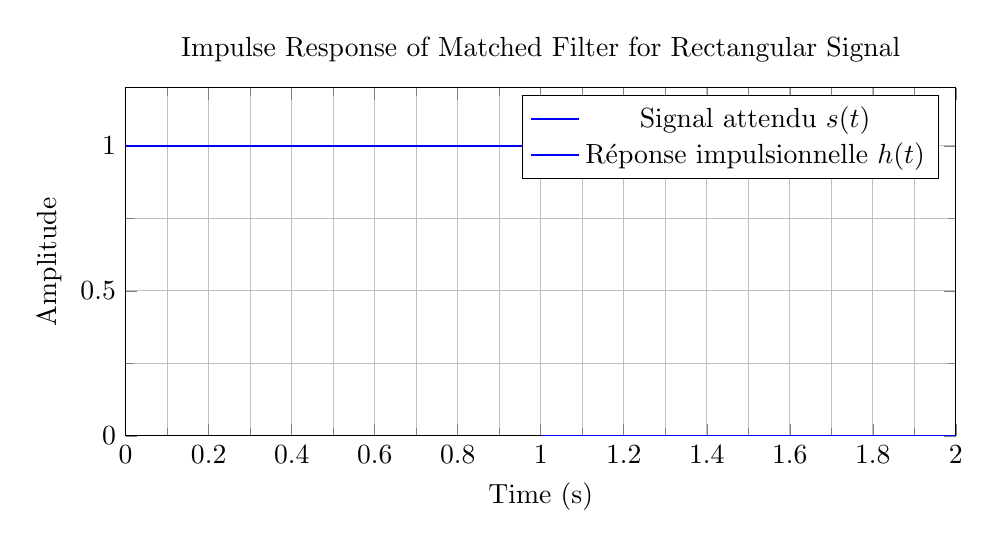
\begin{tikzpicture}
\begin{axis}[
    width=\textwidth,
    height=6cm,
    xlabel=Time (s),
    ylabel=Amplitude,
    title=Impulse Response of Matched Filter for Rectangular Signal,
    xmin=0, xmax=2,
    ymin=0, ymax=1.2,
    grid=both,
    minor tick num=1,
]

\addplot[blue, thick, domain=0:1, samples=100] {1};
\addplot[blue, thick, domain=1:2, samples=2] {0};
\legend{Signal attendu $s(t)$, Réponse impulsionnelle $h(t)$}

\end{axis}
\end{tikzpicture}

\subsection*{Sortie du Filtre Adapté pour un Signal Rectangulaire}
La sortie du filtre adapté pour un signal rectangulaire est un signal triangulaire, qui atteint son maximum à \( t = T \).

\subsection*{Illustration de la Sortie du Filtre Adapté}
Voici un exemple de la sortie du filtre adapté pour un signal rectangulaire :

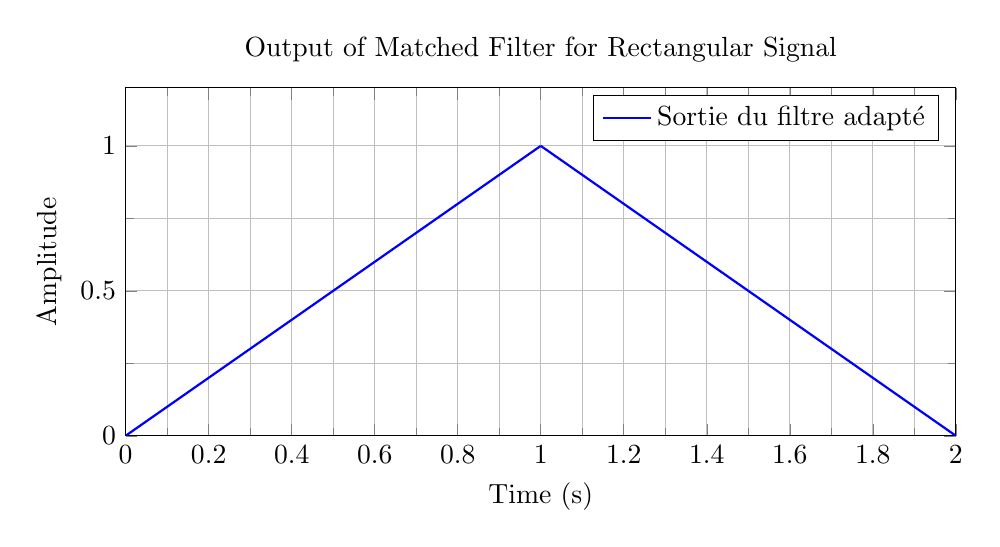
\begin{tikzpicture}
\begin{axis}[
    width=\textwidth,
    height=6cm,
    xlabel=Time (s),
    ylabel=Amplitude,
    title=Output of Matched Filter for Rectangular Signal,
    xmin=0, xmax=2,
    ymin=0, ymax=1.2,
    grid=both,
    minor tick num=1,
]

\addplot[blue, thick, domain=0:1, samples=100] {x};
\addplot[blue, thick, domain=1:2, samples=100] {2-x};
\legend{Sortie du filtre adapté}

\end{axis}
\end{tikzpicture}

\subsection*{Avantages du Filtre Adapté}
- Maximisation du SNR à l'instant de décision.
- Réduction de la probabilité d'erreur.
- Facilité de mise en œuvre dans les systèmes numériques.

\subsection*{Application aux Modulations Numériques}
Le filtre adapté est utilisé dans divers systèmes de modulation numérique, tels que :
- BPSK (Binary Phase Shift Keying)
- QPSK (Quadrature Phase Shift Keying)
- QAM (Quadrature Amplitude Modulation)

\subsection*{Exemple d'Application en BPSK}
Pour un système BPSK, le filtre adapté est conçu pour correspondre à la forme d'onde du symbole BPSK. Cela permet de maximiser le SNR et de minimiser la probabilité d'erreur.

\subsection*{Conclusion}
Le filtre adapté est un outil essentiel dans les systèmes de communication numérique. Il permet de maximiser le rapport signal sur bruit à l'instant de décision, ce qui améliore la détection des symboles et réduit la probabilité d'erreur. Les illustrations et explications présentés montrent comment le filtre adapté fonctionne et comment il peut être appliqué à différents types de modulations numériques.

\section*{Vector Representation}

\subsection*{Introduction}
La représentation vectorielle des signaux est une méthode puissante pour analyser et concevoir des systèmes de communication. Elle permet de représenter les signaux comme des vecteurs dans un espace de dimension finie, facilitant ainsi l'analyse des performances et la détection des symboles.

\subsection*{Espace de Signal}
Un espace de signal est un espace vectoriel où chaque signal est représenté par un vecteur. Les bases de cet espace sont généralement des fonctions orthogonales.

\subsection*{Base Orthonormée}
Une base orthonormée est un ensemble de fonctions \(\{\phi_i(t)\}\) telles que :
\[
\int_{0}^{T} \phi_i(t) \phi_j(t) \, dt = \begin{cases}
1 & \text{si } i = j \\
0 & \text{si } i \neq j
\end{cases}
\]
où \(T\) est la durée du symbole.

\subsection*{Représentation Vectorielle d'un Signal}
Un signal \(s(t)\) peut être représenté dans une base orthonormée \(\{\phi_i(t)\}\) comme :
\[
s(t) = \sum_{i=1}^{N} s_i \phi_i(t)
\]
où \(s_i\) sont les composantes du vecteur représentant le signal \(s(t)\).

\subsection*{Exemple de Base Orthonormée}
Pour un signal binaire, une base orthonormée simple peut être :
\[
\phi_1(t) = \sqrt{\frac{2}{T}} \cos(2\pi f_0 t), \quad \phi_2(t) = \sqrt{\frac{2}{T}} \sin(2\pi f_0 t)
\]
où \(f_0\) est la fréquence de la porteuse.

\subsection*{Illustration de la Base Orthonormée}
Voici un exemple de deux fonctions de base orthonormées :

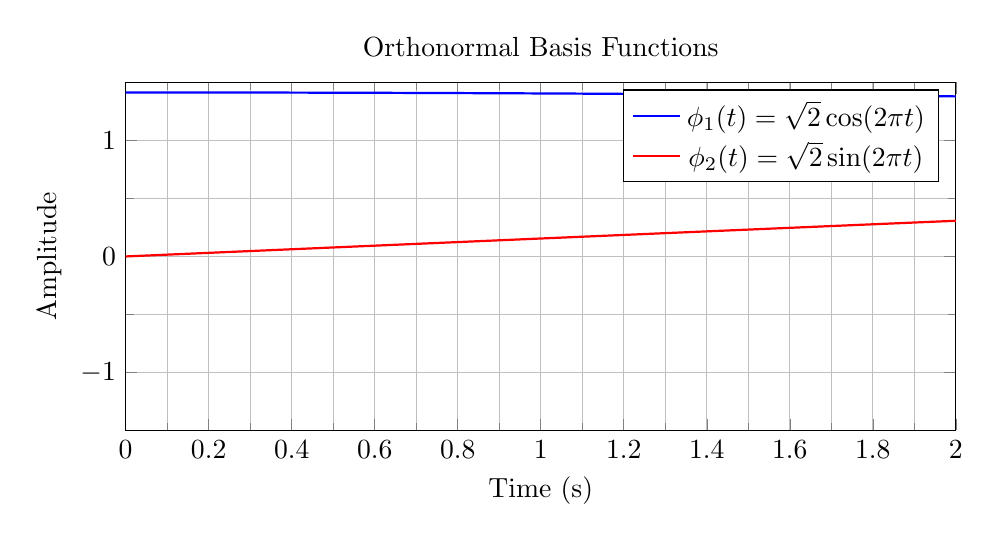
\begin{tikzpicture}
\begin{axis}[
    width=\textwidth,
    height=6cm,
    xlabel=Time (s),
    ylabel=Amplitude,
    title=Orthonormal Basis Functions,
    xmin=0, xmax=2,
    ymin=-1.5, ymax=1.5,
    grid=both,
    minor tick num=1,
]

\addplot[blue, thick, domain=0:2, samples=100] {sqrt(2)*cos(2*pi*x)};
\addplot[red, thick, domain=0:2, samples=100] {sqrt(2)*sin(2*pi*x)};
\legend{$\phi_1(t) = \sqrt{2} \cos(2\pi t)$, $\phi_2(t) = \sqrt{2} \sin(2\pi t)$}

\end{axis}
\end{tikzpicture}

\subsection*{Constellation de Signaux}
La constellation de signaux est une représentation graphique des vecteurs de signal dans l'espace de signal. Chaque point de la constellation correspond à un symbole.

\subsection*{Exemple de Constellation pour BPSK}
Pour une modulation BPSK, la constellation est composée de deux points :
\[
s_0(t) = -\sqrt{E_b} \phi_1(t), \quad s_1(t) = +\sqrt{E_b} \phi_1(t)
\]
où \(E_b\) est l'énergie par bit.

\subsection*{Illustration de la Constellation BPSK}
Voici un exemple de constellation pour BPSK :

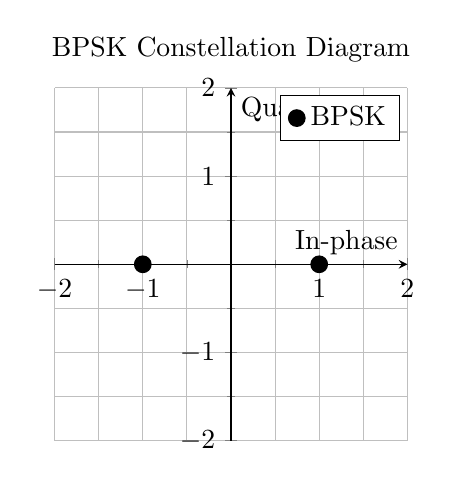
\begin{tikzpicture}
\begin{axis}[
    width=0.5\textwidth,
    height=0.5\textwidth,
    xlabel=In-phase,
    ylabel=Quadrature,
    title=BPSK Constellation Diagram,
    xmin=-2, xmax=2,
    ymin=-2, ymax=2,
    grid=both,
    minor tick num=1,
    axis lines=middle,
]

\addplot[only marks, mark=*, mark size=3pt] coordinates {
    (-1, 0)
    (1, 0)
};
\legend{BPSK}

\end{axis}
\end{tikzpicture}

\subsection*{Exemple de Constellation pour QPSK}
Pour une modulation QPSK, la constellation est composée de quatre points :
\[
\begin{aligned}
s_0(t) &= +\sqrt{\frac{E_s}{2}} \phi_1(t) + \sqrt{\frac{E_s}{2}} \phi_2(t) \\
s_1(t) &= -\sqrt{\frac{E_s}{2}} \phi_1(t) + \sqrt{\frac{E_s}{2}} \phi_2(t) \\
s_2(t) &= -\sqrt{\frac{E_s}{2}} \phi_1(t) - \sqrt{\frac{E_s}{2}} \phi_2(t) \\
s_3(t) &= +\sqrt{\frac{E_s}{2}} \phi_1(t) - \sqrt{\frac{E_s}{2}} \phi_2(t)
\end{aligned}
\]
où \(E_s\) est l'énergie par symbole.

\subsection*{Illustration de la Constellation QPSK}
Voici un exemple de constellation pour QPSK :

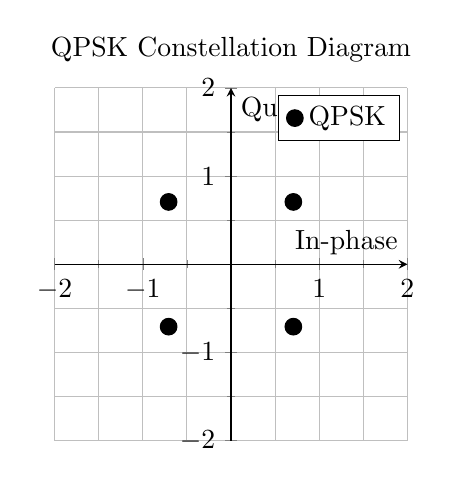
\begin{tikzpicture}
\begin{axis}[
    width=0.5\textwidth,
    height=0.5\textwidth,
    xlabel=In-phase,
    ylabel=Quadrature,
    title=QPSK Constellation Diagram,
    xmin=-2, xmax=2,
    ymin=-2, ymax=2,
    grid=both,
    minor tick num=1,
    axis lines=middle,
]

\addplot[only marks, mark=*, mark size=3pt] coordinates {
    (0.707, 0.707)
    (-0.707, 0.707)
    (-0.707, -0.707)
    (0.707, -0.707)
};
\legend{QPSK}

\end{axis}
\end{tikzpicture}

\subsection*{Avantages de la Représentation Vectorielle}
- **Simplification de l'analyse** : La représentation vectorielle permet de simplifier l'analyse des systèmes de communication.
- **Visualisation des signaux** : Les constellations permettent de visualiser les signaux et de comprendre les relations entre les symboles.
- **Optimisation des performances** : Elle facilite l'optimisation des performances en termes de probabilité d'erreur et d'efficacité spectrale.

\subsection*{Distance Euclidienne}
La distance euclidienne entre deux vecteurs de signal est une mesure de leur séparation dans l'espace de signal. Une plus grande distance euclidienne entre les points de la constellation réduit la probabilité d'erreur.

\subsection*{Exemple de Distance Euclidienne pour BPSK}
Pour BPSK, la distance euclidienne entre les deux points de la constellation est :
\[
d = 2\sqrt{E_b}
\]

\subsection*{Exemple de Distance Euclidienne pour QPSK}
Pour QPSK, la distance euclidienne entre deux points adjacents de la constellation est :
\[
d = \sqrt{2E_s}
\]

\subsection*{Conclusion}
La représentation vectorielle des signaux est un outil essentiel pour l'analyse et la conception des systèmes de communication numérique. Elle permet de simplifier l'analyse des performances, de visualiser les signaux et d'optimiser les systèmes en termes de probabilité d'erreur et d'efficacité spectrale. Les illustrations et explications présentées montrent comment les signaux peuvent être représentés dans un espace vectoriel et comment cette représentation peut être utilisée pour améliorer les performances des systèmes de communication.

\section*{Analog Modulation}

\subsection*{Introduction}
La modulation analogique est une technique utilisée pour transmettre des signaux analogiques (comme la voix ou la musique) sur des canaux de communication. Elle consiste à modifier une onde porteuse en fonction du signal à transmettre.

\subsection*{Types de Modulation Analogique}
Il existe principalement trois types de modulation analogique :
\begin{itemize}
    \item **Amplitude Modulation (AM)** : L'amplitude de la porteuse est modifiée en fonction du signal.
    \item **Frequency Modulation (FM)** : La fréquence de la porteuse est modifiée en fonction du signal.
    \item **Phase Modulation (PM)** : La phase de la porteuse est modifiée en fonction du signal.
\end{itemize}

\subsection*{Amplitude Modulation (AM)}
Dans la modulation d'amplitude, l'amplitude de la porteuse est proportionnelle au signal modulant.

\subsubsection*{Expression Mathématique}
Un signal AM peut être exprimé comme :
\[ s_{AM}(t) = A_c \left[1 + m(t)\right] \cos(2\pi f_c t) \]
où :
- \( A_c \) est l'amplitude de la porteuse,
- \( m(t) \) est le signal modulant,
- \( f_c \) est la fréquence de la porteuse.

\subsubsection*{Indice de Modulation}
L'indice de modulation \( \mu \) est défini comme :
\[ \mu = \frac{A_m}{A_c} \]
où \( A_m \) est l'amplitude maximale du signal modulant.

\subsubsection*{Spectre du Signal AM}
Le spectre d'un signal AM contient la fréquence de la porteuse et les bandes latérales :
\[ S_{AM}(f) = \frac{A_c}{2} \left[ \delta(f - f_c) + \delta(f + f_c) \right] + \frac{A_c}{2} \left[ M(f - f_c) + M(f + f_c) \right] \]
où \( M(f) \) est la transformée de Fourier du signal modulant \( m(t) \).

\subsubsection*{Illustration du Signal AM}
Voici un exemple de signal AM :

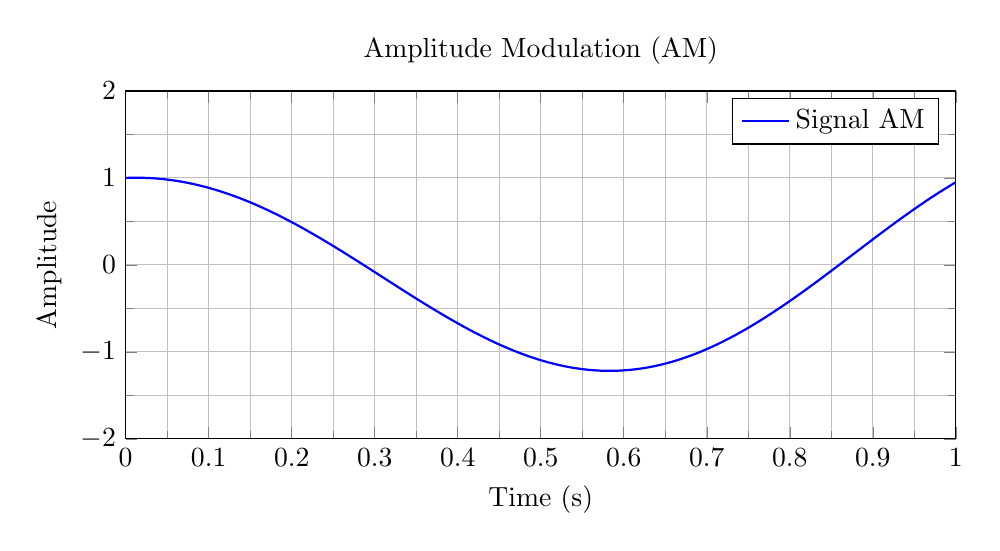
\begin{tikzpicture}
\begin{axis}[
    width=\textwidth,
    height=6cm,
    xlabel=Time (s),
    ylabel=Amplitude,
    title=Amplitude Modulation (AM),
    xmin=0, xmax=1,
    ymin=-2, ymax=2,
    grid=both,
    minor tick num=1,
]

\addplot[blue, thick, domain=0:1, samples=200] {(1+0.7*sin(2*pi*5*x))*cos(2*pi*50*x)};
\legend{Signal AM}

\end{axis}
\end{tikzpicture}

\subsection*{Frequency Modulation (FM)}
Dans la modulation de fréquence, la fréquence de la porteuse est modifiée en fonction du signal modulant.

\subsubsection*{Expression Mathématique}
Un signal FM peut être exprimé comme :
\[ s_{FM}(t) = A_c \cos \left(2\pi f_c t + 2\pi k_f \int_{0}^{t} m(\tau) \, d\tau \right) \]
où :
- \( A_c \) est l'amplitude de la porteuse,
- \( k_f \) est la constante de déviation de fréquence,
- \( m(t) \) est le signal modulant.

\subsubsection*{Indice de Modulation pour FM}
L'indice de modulation \( \beta \) est défini comme :
\[ \beta = \frac{\Delta f}{f_m} \]
où \( \Delta f \) est la déviation maximale de fréquence et \( f_m \) est la fréquence maximale du signal modulant.

\subsubsection*{Spectre du Signal FM}
Le spectre d'un signal FM est plus complexe que celui d'un signal AM et contient une infinité de bandes latérales. Cependant, pour un indice de modulation \( \beta \) donné, la bande passante peut être approximée par la règle de Carson :
\[ B = 2(\beta + 1)f_m \]

\subsubsection*{Illustration du Signal FM}
Voici un exemple de signal FM :

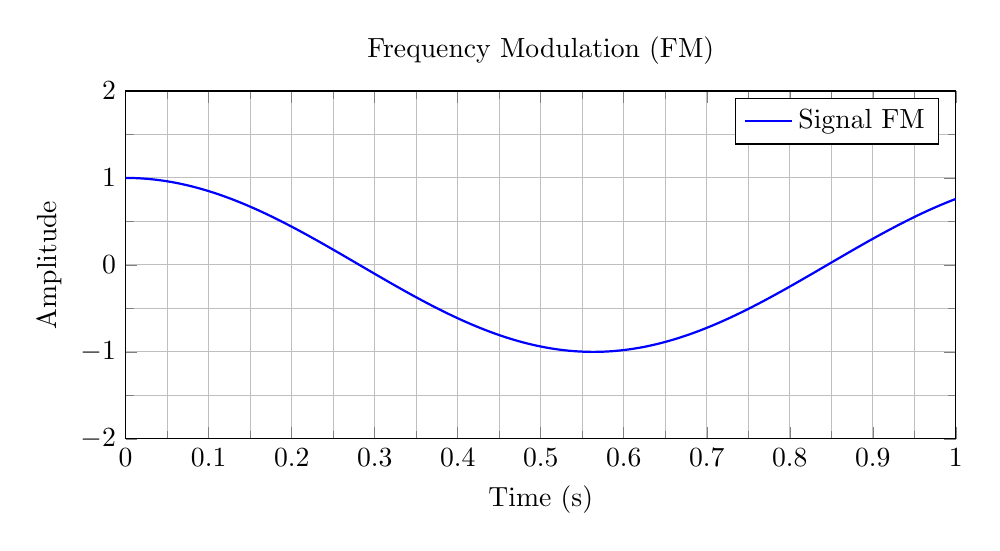
\begin{tikzpicture}
\begin{axis}[
    width=\textwidth,
    height=6cm,
    xlabel=Time (s),
    ylabel=Amplitude,
    title=Frequency Modulation (FM),
    xmin=0, xmax=1,
    ymin=-2, ymax=2,
    grid=both,
    minor tick num=1,
]

\pgfmathsetseed{1}
\addplot[blue, thick, domain=0:1, samples=200] {cos(2*pi*50*x + 10*sin(2*pi*5*x))};
\legend{Signal FM}

\end{axis}
\end{tikzpicture}

\subsection*{Phase Modulation (PM)}
Dans la modulation de phase, la phase de la porteuse est modifiée en fonction du signal modulant.

\subsubsection*{Expression Mathématique}
Un signal PM peut être exprimé comme :
\[ s_{PM}(t) = A_c \cos \left(2\pi f_c t + k_p m(t) \right) \]
où :
- \( A_c \) est l'amplitude de la porteuse,
- \( k_p \) est la constante de déviation de phase,
- \( m(t) \) est le signal modulant.

\subsubsection*{Indice de Modulation pour PM}
L'indice de modulation pour PM est similaire à celui de FM, mais il est basé sur la déviation de phase.

\subsection*{Comparaison des Modulations Analogiques}
Voici un tableau comparatif des différentes modulations analogiques :

\begin{tabular}{|c|c|c|}
\hline
Type de Modulation & Avantages & Inconvénients \\
\hline
AM & Simplicité de mise en œuvre, faible bande passante & Sensible au bruit et aux interférences \\
\hline
FM & Meilleure résistance au bruit, meilleure qualité audio & Bande passante plus large \\
\hline
PM & Moins sensible au bruit que AM & Complexité de mise en œuvre \\
\hline
\end{tabular}

\subsection*{Applications des Modulations Analogiques}
- **AM** : Utilisée dans la radio AM, la télévision analogique.
- **FM** : Utilisée dans la radio FM, les communications audio de haute qualité.
- **PM** : Utilisée dans certaines applications de communication où la phase est plus facile à contrôler.

\subsection*{Conclusion}
La modulation analogique est une technique essentielle pour transmettre des signaux analogiques sur des canaux de communication. Les trois principaux types de modulation analogique (AM, FM, PM) ont chacun leurs avantages et inconvénients, et sont utilisés dans diverses applications en fonction des besoins spécifiques en termes de qualité, de bande passante et de résistance au bruit.

\section*{Digital Modulation}

\subsection*{Introduction}
La modulation numérique est une technique utilisée pour transmettre des données numériques en modifiant une onde porteuse. Contrairement à la modulation analogique, elle manipule des signaux discrets, ce qui permet une meilleure résistance au bruit et une efficacité spectrale accrue.

\subsection*{Types de Modulation Numérique}
Il existe plusieurs types de modulation numérique, parmi lesquels :
\begin{itemize}
    \item **Amplitude Shift Keying (ASK)**
    \item **Frequency Shift Keying (FSK)**
    \item **Phase Shift Keying (PSK)**
    \item **Quadrature Amplitude Modulation (QAM)**
\end{itemize}

\subsection*{Amplitude Shift Keying (ASK)}
Dans la modulation ASK, l'amplitude de la porteuse est modifiée pour représenter les données numériques.

\subsubsection*{Expression Mathématique}
Un signal ASK peut être exprimé comme :
\[ s_{ASK}(t) = A_i \cos(2\pi f_c t) \]
où \( A_i \) prend des valeurs discrètes en fonction des bits à transmettre, et \( f_c \) est la fréquence de la porteuse.

\subsubsection*{Exemple de Signal ASK}
Pour un signal binaire, \( A_i \) peut prendre deux valeurs, par exemple 0 et \( A \).

\subsubsection*{Illustration du Signal ASK}
Voici un exemple de signal ASK pour une séquence binaire :

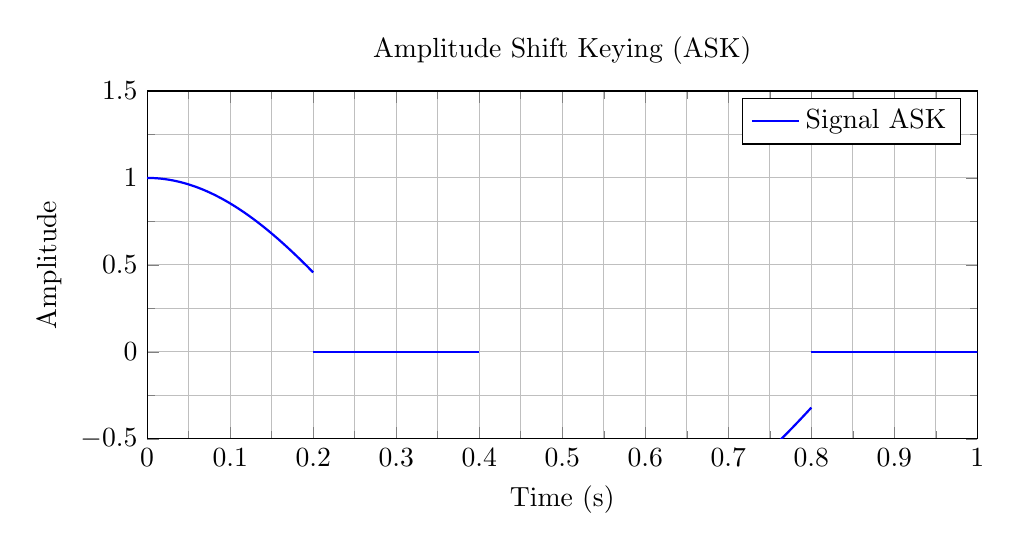
\begin{tikzpicture}
\begin{axis}[
    width=\textwidth,
    height=6cm,
    xlabel=Time (s),
    ylabel=Amplitude,
    title=Amplitude Shift Keying (ASK),
    xmin=0, xmax=1,
    ymin=-0.5, ymax=1.5,
    grid=both,
    minor tick num=1,
]

\addplot[blue, thick, domain=0:0.2, samples=200] {1*cos(2*pi*50*x)};
\addplot[blue, thick, domain=0.2:0.4, samples=200] {0*cos(2*pi*50*x)};
\addplot[blue, thick, domain=0.4:0.6, samples=200] {1*cos(2*pi*50*x)};
\addplot[blue, thick, domain=0.6:0.8, samples=200] {1*cos(2*pi*50*x)};
\addplot[blue, thick, domain=0.8:1, samples=200] {0*cos(2*pi*50*x)};
\legend{Signal ASK}

\end{axis}
\end{tikzpicture}

\subsection*{Frequency Shift Keying (FSK)}
Dans la modulation FSK, la fréquence de la porteuse est modifiée pour représenter les données numériques.

\subsubsection*{Expression Mathématique}
Un signal FSK peut être exprimé comme :
\[ s_{FSK}(t) = A \cos(2\pi f_i t) \]
où \( f_i \) prend des valeurs discrètes en fonction des bits à transmettre.

\subsubsection*{Exemple de Signal FSK}
Pour un signal binaire, \( f_i \) peut prendre deux valeurs, par exemple \( f_0 \) et \( f_1 \).

\subsubsection*{Illustration du Signal FSK}
Voici un exemple de signal FSK pour une séquence binaire :

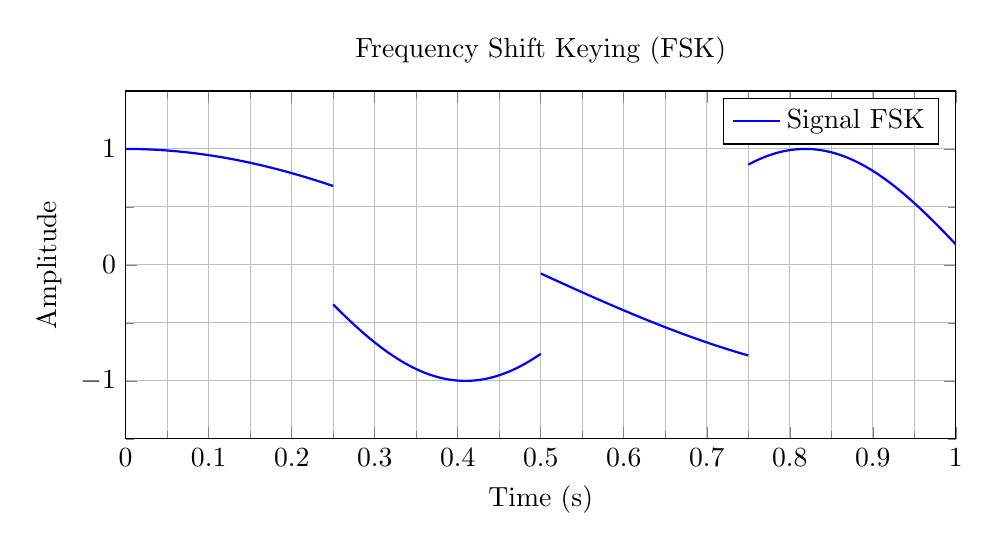
\begin{tikzpicture}
\begin{axis}[
    width=\textwidth,
    height=6cm,
    xlabel=Time (s),
    ylabel=Amplitude,
    title=Frequency Shift Keying (FSK),
    xmin=0, xmax=1,
    ymin=-1.5, ymax=1.5,
    grid=both,
    minor tick num=1,
]

\addplot[blue, thick, domain=0:0.25, samples=200] {cos(2*pi*30*x)};
\addplot[blue, thick, domain=0.25:0.5, samples=200] {cos(2*pi*70*x)};
\addplot[blue, thick, domain=0.5:0.75, samples=200] {cos(2*pi*30*x)};
\addplot[blue, thick, domain=0.75:1, samples=200] {cos(2*pi*70*x)};
\legend{Signal FSK}

\end{axis}
\end{tikzpicture}

\subsection*{Phase Shift Keying (PSK)}
Dans la modulation PSK, la phase de la porteuse est modifiée pour représenter les données numériques.

\subsubsection*{Expression Mathématique}
Un signal PSK peut être exprimé comme :
\[ s_{PSK}(t) = A \cos(2\pi f_c t + \theta_i) \]
où \( \theta_i \) prend des valeurs discrètes en fonction des bits à transmettre.

\subsubsection*{Exemple de Signal BPSK}
Pour un signal BPSK (Binary PSK), \( \theta_i \) peut prendre deux valeurs, par exemple 0 et \( \pi \).

\subsubsection*{Illustration du Signal BPSK}
Voici un exemple de signal BPSK pour une séquence binaire :

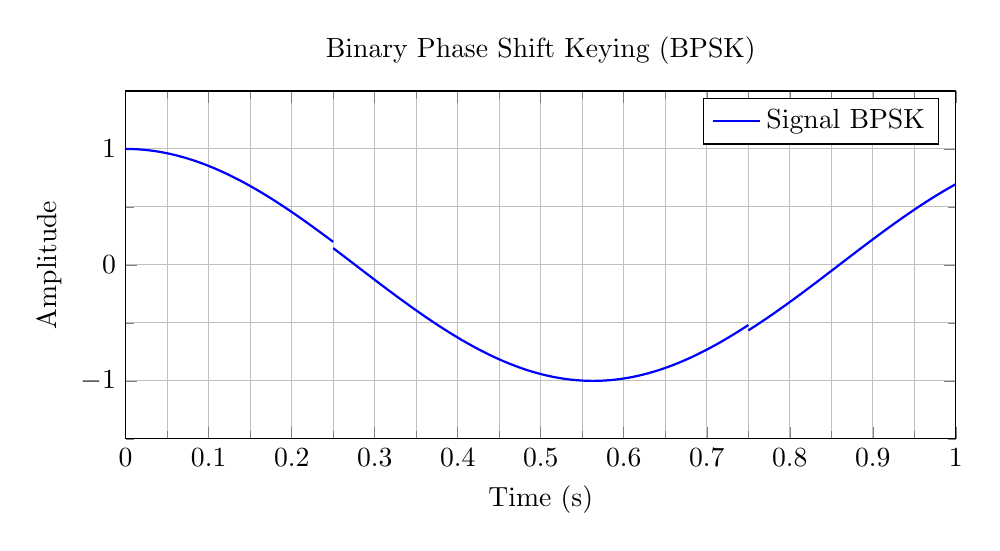
\begin{tikzpicture}
\begin{axis}[
    width=\textwidth,
    height=6cm,
    xlabel=Time (s),
    ylabel=Amplitude,
    title=Binary Phase Shift Keying (BPSK),
    xmin=0, xmax=1,
    ymin=-1.5, ymax=1.5,
    grid=both,
    minor tick num=1,
]

\addplot[blue, thick, domain=0:0.25, samples=200] {cos(2*pi*50*x)};
\addplot[blue, thick, domain=0.25:0.5, samples=200] {cos(2*pi*50*x + pi)};
\addplot[blue, thick, domain=0.5:0.75, samples=200] {cos(2*pi*50*x + pi)};
\addplot[blue, thick, domain=0.75:1, samples=200] {cos(2*pi*50*x)};
\legend{Signal BPSK}

\end{axis}
\end{tikzpicture}

\subsection*{Quadrature Amplitude Modulation (QAM)}
La modulation QAM combine la modulation d'amplitude et de phase pour représenter les données numériques.

\subsubsection*{Expression Mathématique}
Un signal QAM peut être exprimé comme :
\[ s_{QAM}(t) = A_i \cos(2\pi f_c t) + B_i \sin(2\pi f_c t) \]
où \( A_i \) et \( B_i \) prennent des valeurs discrètes en fonction des bits à transmettre.

\subsubsection*{Exemple de Signal 16-QAM}
Pour un signal 16-QAM, il y a 16 combinaisons possibles de \( A_i \) et \( B_i \).

\subsubsection*{Illustration de la Constellation 16-QAM}
Voici un exemple de constellation pour 16-QAM :

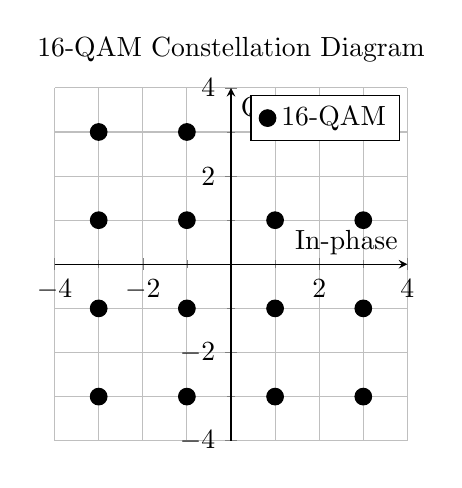
\begin{tikzpicture}
\begin{axis}[
    width=0.5\textwidth,
    height=0.5\textwidth,
    xlabel=In-phase,
    ylabel=Quadrature,
    title=16-QAM Constellation Diagram,
    xmin=-4, xmax=4,
    ymin=-4, ymax=4,
    grid=both,
    minor tick num=1,
    axis lines=middle,
]

\addplot[only marks, mark=*, mark size=3pt] coordinates {
    (-3, -3) (-3, -1) (-3, 1) (-3, 3)
    (-1, -3) (-1, -1) (-1, 1) (-1, 3)
    (1, -3) (1, -1) (1, 1) (1, 3)
    (3, -3) (3, -1) (3, 1) (3, 3)
};
\legend{16-QAM}

\end{axis}
\end{tikzpicture}

\subsection*{Avantages de la Modulation Numérique}
- **Résistance au bruit** : Meilleure résistance au bruit et aux interférences.
- **Efficacité spectrale** : Meilleure utilisation de la bande passante.
- **Flexibilité** : Possibilité de choisir parmi plusieurs types de modulations en fonction des besoins.

\subsection*{Comparaison des Modulations Numériques}
Voici un tableau comparatif des différentes modulations numériques :

\begin{tabular}{|c|c|c|}
\hline
Type de Modulation & Avantages & Inconvénients \\
\hline
ASK & Simplicité de mise en œuvre & Sensible aux variations d'amplitude \\
\hline
FSK & Résistance au bruit & Bande passante plus large \\
\hline
PSK & Bonne efficacité spectrale & Sensible aux erreurs de phase \\
\hline
QAM & Haute efficacité spectrale & Complexité de mise en œuvre \\
\hline
\end{tabular}

\subsection*{Applications des Modulations Numériques}
- **ASK** : Utilisée dans les communications optiques et certaines transmissions radio.
- **FSK** : Utilisée dans les communications radio à basse fréquence et les systèmes de télécommande.
- **PSK** : Utilisée dans les systèmes Wi-Fi, Bluetooth, et les communications par satellite.
- **QAM** : Utilisée dans les modems, les systèmes de télévision numérique, et les communications cellulaires (4G, 5G).

\subsection*{Conclusion}
La modulation numérique est une technique essentielle pour transmettre des données numériques de manière efficace et fiable. Les différents types de modulation numérique (ASK, FSK, PSK, QAM) ont chacun leurs avantages et inconvénients, et sont utilisés dans diverses applications en fonction des besoins spécifiques en termes de qualité, de bande passante et de résistance au bruit.

\section*{Filtering of Modulated Signals}

\subsection*{Introduction}
Le filtrage des signaux modulés est une étape essentielle dans les systèmes de communication. Il permet de limiter la bande passante des signaux, de réduire les interférences, et d'optimiser les performances globales du système.

\subsection*{Objectifs du Filtrage}
Les principaux objectifs du filtrage des signaux modulés sont :
\begin{itemize}
    \item **Limitation de la bande passante** : Réduire la largeur de bande du signal pour éviter les interférences avec d'autres signaux.
    \item **Réduction de l'ISI** : Minimiser l'interférence entre symboles.
    \item **Amélioration du SNR** : Augmenter le rapport signal sur bruit.
\end{itemize}

\subsection*{Types de Filtres}
Plusieurs types de filtres peuvent être utilisés pour les signaux modulés :
\begin{itemize}
    \item **Filtre passe-bas** : Utilisé pour éliminer les hautes fréquences.
    \item **Filtre passe-haut** : Utilisé pour éliminer les basses fréquences.
    \item **Filtre passe-bande** : Utilisé pour isoler une bande de fréquences spécifique.
    \item **Filtre en cosinus surélevé** : Utilisé pour réduire l'ISI.
\end{itemize}

\subsection*{Filtre Passe-Bas}
Un filtre passe-bas permet de laisser passer les basses fréquences tout en atténuant les hautes fréquences.

\subsubsection*{Réponse en Fréquence}
La réponse en fréquence d'un filtre passe-bas idéal est donnée par :
\[ H(f) = \begin{cases}
1 & \text{si } |f| \leq f_c \\
0 & \text{si } |f| > f_c
\end{cases} \]
où \( f_c \) est la fréquence de coupure.

\subsubsection*{Illustration de la Réponse en Fréquence d'un Filtre Passe-Bas}
Voici un exemple de réponse en fréquence d'un filtre passe-bas idéal :

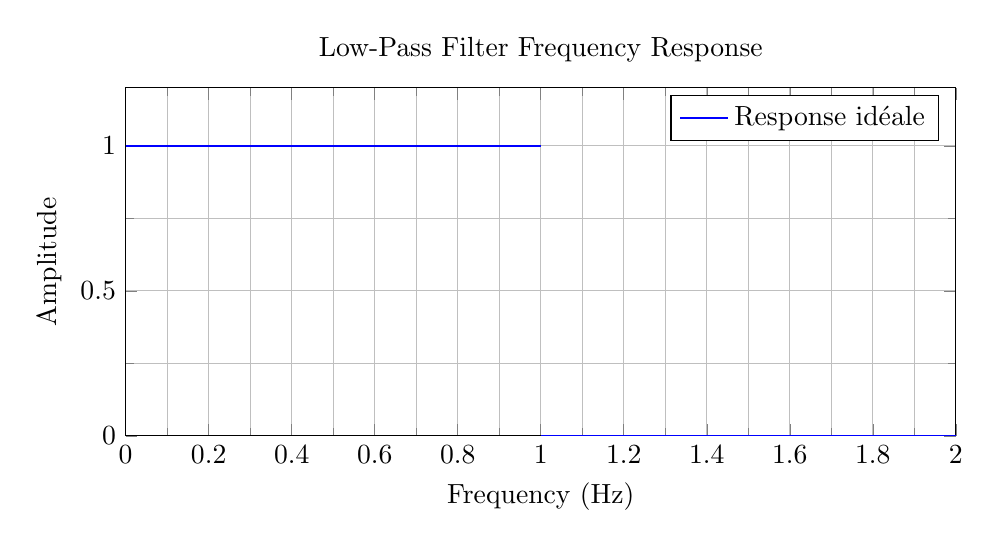
\begin{tikzpicture}
\begin{axis}[
    width=\textwidth,
    height=6cm,
    xlabel=Frequency (Hz),
    ylabel=Amplitude,
    title=Low-Pass Filter Frequency Response,
    xmin=0, xmax=2,
    ymin=0, ymax=1.2,
    grid=both,
    minor tick num=1,
]

\addplot[blue, thick, domain=0:1, samples=100] {1};
\addplot[blue, thick, domain=1:2, samples=2] {0};
\legend{Response idéale}

\end{axis}
\end{tikzpicture}

\subsection*{Filtre en Cosinus Surélevé}
Le filtre en cosinus surélevé est couramment utilisé dans les systèmes de communication numérique pour réduire l'ISI.

\subsubsection*{Réponse en Fréquence}
La réponse en fréquence d'un filtre en cosinus surélevé est donnée par :
\[ H(f) = \begin{cases}
1 & \text{si } |f| < \frac{1 - \alpha}{2T_s} \\
\frac{1}{2} \left[1 + \cos\left(\frac{\pi T_s}{\alpha} \left(|f| - \frac{1 - \alpha}{2T_s}\right)\right)\right] & \text{si } \frac{1 - \alpha}{2T_s} < |f| < \frac{1 + \alpha}{2T_s} \\
0 & \text{sinon}
\end{cases} \]
où \( T_s \) est la période des symboles et \( \alpha \) est le facteur de roll-off.

\subsubsection*{Illustration de la Réponse en Fréquence d'un Filtre en Cosinus Surélevé}
Voici un exemple de réponse en fréquence d'un filtre en cosinus surélevé avec un facteur de roll-off \( \alpha = 0.5 \) :

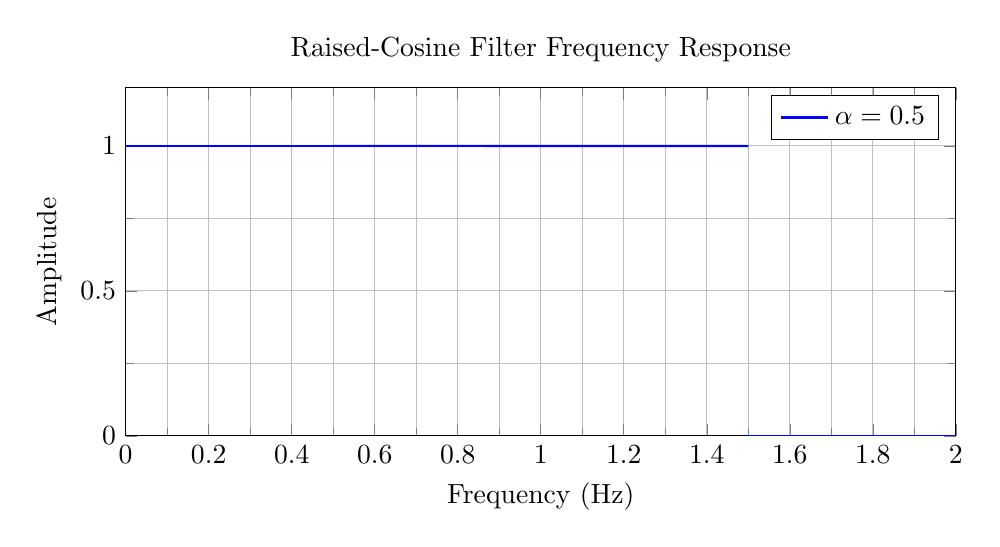
\begin{tikzpicture}
\begin{axis}[
    width=\textwidth,
    height=6cm,
    xlabel=Frequency (Hz),
    ylabel=Amplitude,
    title=Raised-Cosine Filter Frequency Response,
    xmin=0, xmax=2,
    ymin=0, ymax=1.2,
    grid=both,
    minor tick num=1,
]

\addplot[blue, thick, domain=0:0.5, samples=100] {1};
\addplot[blue, thick, domain=0.5:1.5, samples=100] {0.5*(1 + cos(pi*(x-0.5)))};
\addplot[blue, thick, domain=1.5:2, samples=2] {0};
\legend{$\alpha = 0.5$}

\end{axis}
\end{tikzpicture}

\subsection*{Filtre Adapté}
Le filtre adapté est utilisé pour maximiser le rapport signal sur bruit à l'instant de décision.

\subsubsection*{Réponse Impulsionnelle}
La réponse impulsionnelle d'un filtre adapté est donnée par :
\[ h(t) = s(T - t) \]
où \( s(t) \) est le signal attendu et \( T \) est la durée du symbole.

\subsection*{Filtrage des Signaux ASK}
Pour les signaux ASK, le filtrage est utilisé pour éliminer les composantes de fréquence indésirables et pour améliorer la détection des symboles.

\subsubsection*{Exemple de Filtrage ASK}
Un filtre passe-bas peut être utilisé pour éliminer les hautes fréquences et réduire le bruit.

\subsection*{Filtrage des Signaux FSK}
Pour les signaux FSK, le filtrage est utilisé pour isoler les différentes fréquences porteuses.

\subsubsection*{Exemple de Filtrage FSK}
Un filtre passe-bande peut être utilisé pour chaque fréquence porteuse afin de séparer les différents symboles.

\subsection*{Filtrage des Signaux PSK}
Pour les signaux PSK, le filtrage est utilisé pour réduire l'ISI et améliorer la détection de phase.

\subsubsection*{Exemple de Filtrage PSK}
Un filtre en cosinus surélevé est souvent utilisé pour les signaux PSK afin de limiter la bande passante et réduire l'ISI.

\subsection*{Filtrage des Signaux QAM}
Pour les signaux QAM, le filtrage est utilisé pour réduire l'ISI et améliorer la détection des symboles.

\subsubsection*{Exemple de Filtrage QAM}
Un filtre en cosinus surélevé est couramment utilisé pour les signaux QAM afin de limiter la bande passante et réduire l'ISI.

\subsection*{Conclusion}
Le filtrage des signaux modulés est une étape cruciale dans les systèmes de communication. Il permet de limiter la bande passante, de réduire les interférences, et d'optimiser les performances globales du système. Les différents types de filtres, tels que les filtres passe-bas, passe-haut, passe-bande, et en cosinus surélevé, sont utilisés en fonction des besoins spécifiques des systèmes de communication.

\section*{BER and SER of Modulated Signals}

\subsection*{Introduction}
Le Taux d'Erreur Binaire (BER) et le Taux d'Erreur Symbole (SER) sont des métriques essentielles pour évaluer les performances des systèmes de communication numérique. Ils mesurent la fréquence à laquelle des erreurs se produisent lors de la transmission des bits ou des symboles.

\subsection*{Taux d'Erreur Binaire (BER)}
Le BER est défini comme le rapport entre le nombre de bits erronés et le nombre total de bits transmis :
\[ \text{BER} = \frac{\text{Nombre de bits erronés}}{\text{Nombre total de bits transmis}} \]

\subsection*{Taux d'Erreur Symbole (SER)}
Le SER est défini comme le rapport entre le nombre de symboles erronés et le nombre total de symboles transmis :
\[ \text{SER} = \frac{\text{Nombre de symboles erronés}}{\text{Nombre total de symboles transmis}} \]

\subsection*{Relation entre BER et SER}
Pour les modulations binaires (comme BPSK), le BER est égal au SER. Pour les modulations M-aires, le SER peut être converti en BER en utilisant des approximations spécifiques à chaque type de modulation.

\subsection*{Calcul du BER pour BPSK}
Pour une modulation BPSK en présence de bruit blanc gaussien additif (AWGN), le BER est donné par :
\[ \text{BER} = Q\left(\sqrt{\frac{2E_b}{N_0}}\right) \]
où \( E_b \) est l'énergie par bit et \( N_0 \) est la densité spectrale de puissance du bruit.

\subsubsection*{Illustration du BER pour BPSK}
Voici un graphique montrant le BER pour BPSK en fonction du rapport \( E_b/N_0 \) :

\begin{tikzpicture}
\begin{axis}[
    width=\textwidth,
    height=6cm,
    xlabel=$E_b/N_0$ (dB),
    ylabel=Bit Error Rate (BER),
    title=BER for BPSK,
    xmin=0, xmax=10,
    ymin=1e-5, ymax=1,
    ymode=log,
    grid=both,
    minor tick num=1,
]



\addplot[blue, thick, domain=0:10, samples=50] {qfunc(sqrt(2*10^(x/10)))};
\legend{BPSK}

\end{axis}
\end{tikzpicture}

\subsection*{Calcul du BER pour QPSK}
Pour une modulation QPSK, le BER est approximé par :
\[ \text{BER} \approx Q\left(\sqrt{\frac{2E_b}{N_0}}\right) \]
où \( E_b \) est l'énergie par bit.

\subsubsection*{Illustration du BER pour QPSK}
Voici un graphique montrant le BER pour QPSK en fonction du rapport \( E_b/N_0 \) :

\begin{tikzpicture}
\begin{axis}[
    width=\textwidth,
    height=6cm,
    xlabel=$E_b/N_0$ (dB),
    ylabel=Bit Error Rate (BER),
    title=BER for QPSK,
    xmin=0, xmax=15,
    ymin=1e-5, ymax=1,
    ymode=log,
    grid=both,
    minor tick num=1,
]

\addplot[blue, thick, domain=0:15, samples=50] {qfunc(sqrt(2*10^(x/10)))};
\legend{QPSK}

\end{axis}
\end{tikzpicture}

\subsection*{Calcul du SER pour M-PSK}
Pour une modulation M-PSK, le SER est donné par :
\[ \text{SER} \approx 2Q\left(\sqrt{\frac{2E_s}{N_0}} \sin\left(\frac{\pi}{M}\right)\right) \]
où \( E_s \) est l'énergie par symbole.

\subsubsection*{Illustration du SER pour M-PSK}
Voici un graphique montrant le SER pour 8-PSK en fonction du rapport \( E_s/N_0 \) :

\begin{tikzpicture}
\begin{axis}[
    width=\textwidth,
    height=6cm,
    xlabel=$E_s/N_0$ (dB),
    ylabel=Symbol Error Rate (SER),
    title=SER for 8-PSK,
    xmin=0, xmax=20,
    ymin=1e-5, ymax=1,
    ymode=log,
    grid=both,
    minor tick num=1,
]

\addplot[blue, thick, domain=0:20, samples=50] {2*qfunc(sqrt(2*10^(x/10))*sin(pi/8))};
\legend{8-PSK}

\end{axis}
\end{tikzpicture}

\subsection*{Calcul du SER pour M-QAM}
Pour une modulation M-QAM, le SER est approximé par :
\[ \text{SER} \approx 4Q\left(\sqrt{\frac{3E_s}{(M-1)N_0}}\right) \]

\subsubsection*{Illustration du SER pour 16-QAM}
Voici un graphique montrant le SER pour 16-QAM en fonction du rapport \( E_s/N_0 \) :

\begin{tikzpicture}
\begin{axis}[
    width=\textwidth,
    height=6cm,
    xlabel=$E_s/N_0$ (dB),
    ylabel=Symbol Error Rate (SER),
    title=SER for 16-QAM,
    xmin=0, xmax=25,
    ymin=1e-5, ymax=1,
    ymode=log,
    grid=both,
    minor tick num=1,
]

\addplot[blue, thick, domain=0:25, samples=50] {4*qfunc(sqrt(3*10^(x/10)/15))};
\legend{16-QAM}

\end{axis}
\end{tikzpicture}

\subsection*{Comparaison des Performances}
Voici un tableau comparatif des performances en termes de BER et SER pour différentes modulations numériques :

\begin{tabular}{|c|c|c|}
\hline
Modulation & BER/SER & Avantages \\
\hline
BPSK & \( Q\left(\sqrt{\frac{2E_b}{N_0}}\right) \) & Robuste, faible complexité \\
\hline
QPSK & \( Q\left(\sqrt{\frac{2E_b}{N_0}}\right) \) & Meilleure efficacité spectrale que BPSK \\
\hline
8-PSK & \( 2Q\left(\sqrt{\frac{2E_s}{N_0}} \sin\left(\frac{\pi}{8}\right)\right) \) & Efficacité spectrale accrue \\
\hline
16-QAM & \( 4Q\left(\sqrt{\frac{3E_s}{15N_0}}\right) \) & Haute efficacité spectrale \\
\hline
\end{tabular}

\subsection*{Facteurs Influant sur le BER et le SER}
Plusieurs facteurs influencent le BER et le SER :
\begin{itemize}
    \item **Rapport Signal sur Bruit (SNR)** : Plus le SNR est élevé, plus le BER/SER est faible.
    \item **Type de Modulation** : Certaines modulations sont plus robustes aux erreurs que d'autres.
    \item **Interférence Entre Symboles (ISI)** : L'ISI peut augmenter le BER/SER.
    \item **Bande Passante** : Une bande passante limitée peut introduire des distorsions et augmenter les erreurs.
\end{itemize}

\subsection*{Conclusion}
Le Taux d'Erreur Binaire (BER) et le Taux d'Erreur Symbole (SER) sont des indicateurs clés pour évaluer les performances des systèmes de communication numérique. Les graphiques et formules présentés permettent de comparer les performances des différentes modulations et de choisir celle qui convient le mieux à une application donnée en fonction des besoins spécifiques en termes de qualité, de bande passante et de résistance au bruit.

\end{document}
